\begin{frame}{Objectives}

\begin{itemize}
\tightlist
\item
  We want to build this
\end{itemize}

\begin{center}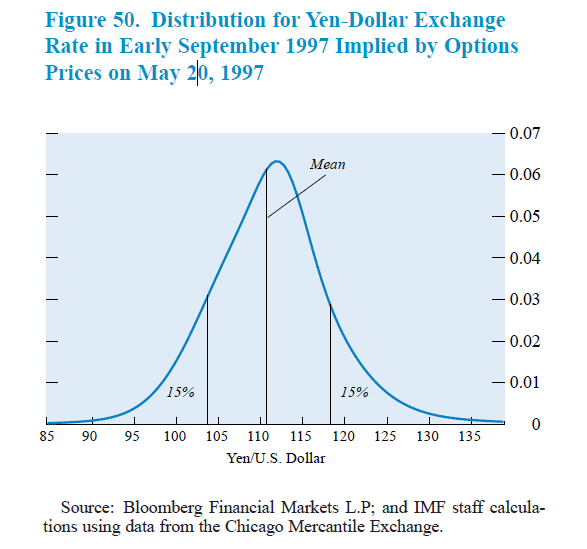
\includegraphics[width=0.6\linewidth]{images/figJPYRND} \end{center}

\end{frame}

\begin{frame}[fragile]{What we will cover}

\begin{itemize}
\tightlist
\item
  Learn about basic FX structures
\item
  Develop some intuition about FX option prices
\item
  Get comfortable with a variety of methods
\item
  Side benefit: learn \texttt{R} and \texttt{RStudio}!
\item
  Lecture notes available at\\
  \color{red} \url{https://jchanlauimf.github.io/IMF_FXOptions}
\end{itemize}

\end{frame}

\begin{frame}{}

\color{blue} \LARGE{Part A:}\\
\LARGE{The Very Basics}

\end{frame}

\begin{frame}{Basics: a plain vanilla call option}

\begin{center}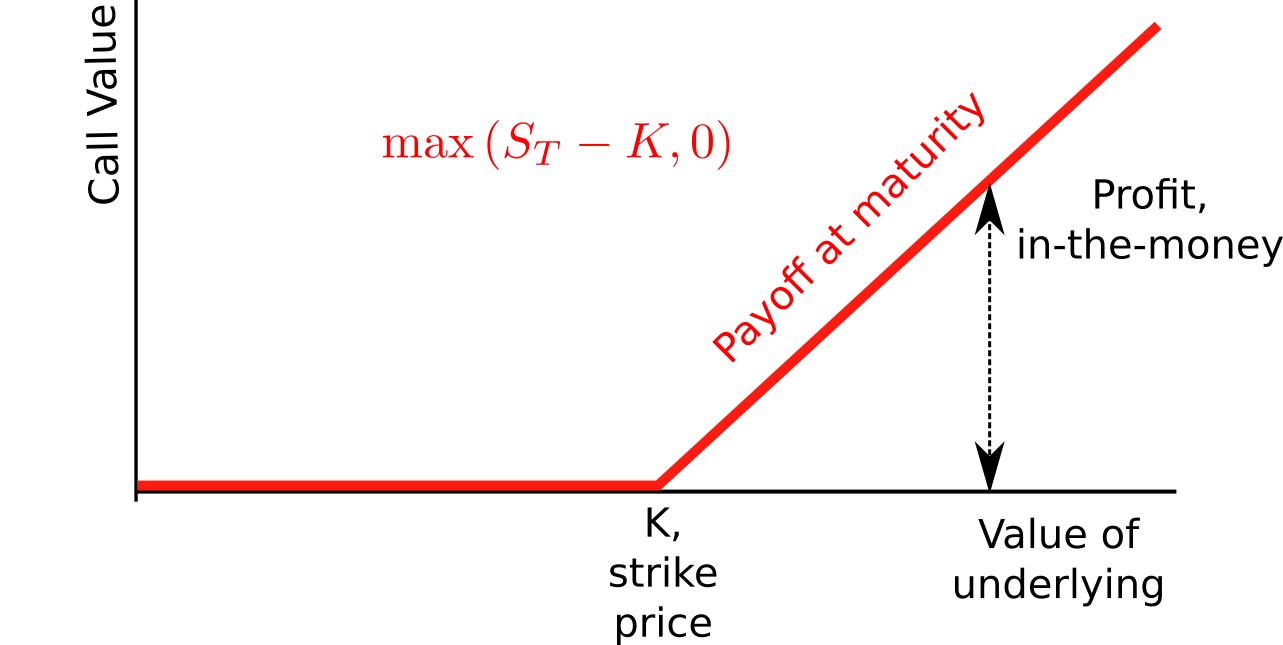
\includegraphics[width=0.8\linewidth]{images/figCallOptionMaturity} \end{center}

\end{frame}

\begin{frame}{Basics: a plain vanilla put option}

\begin{center}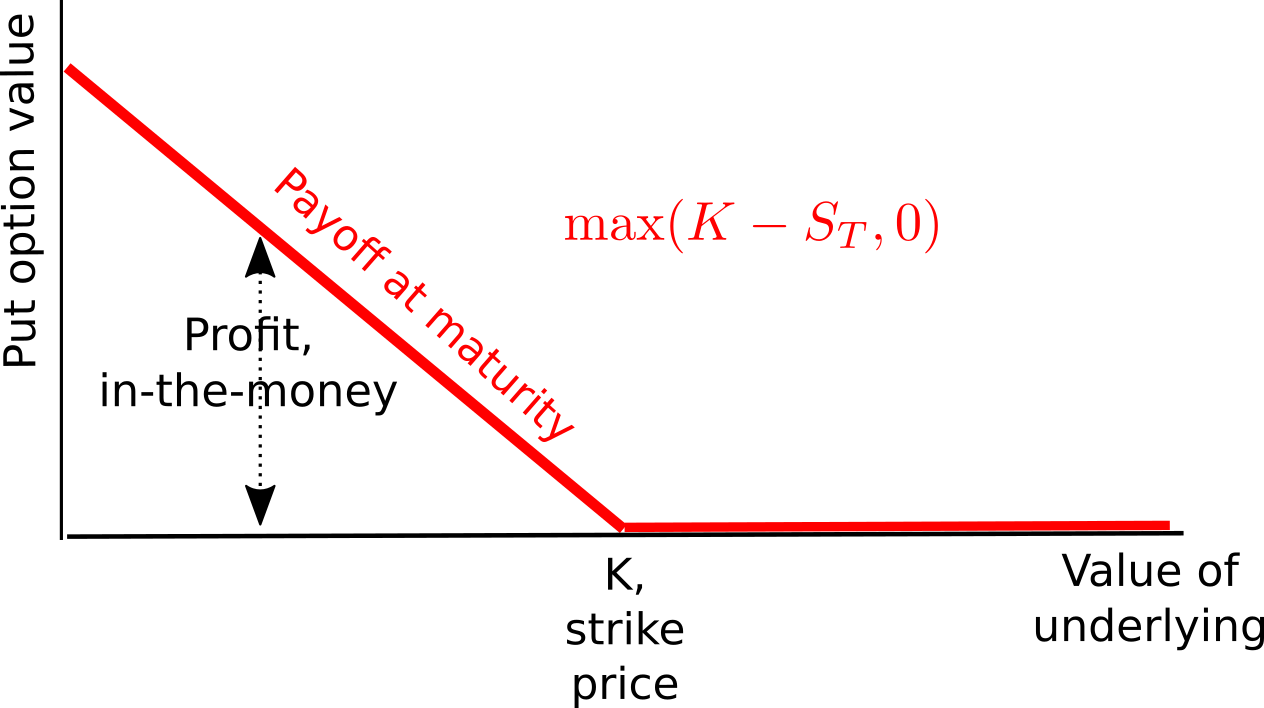
\includegraphics[width=0.8\linewidth]{images/figPutOptionMaturity} \end{center}

\end{frame}

\begin{frame}{Market reality}

\begin{itemize}
\tightlist
\item
  Price quote available for

  \begin{itemize}
  \tightlist
  \item
    ATM plain options
  \end{itemize}
\item
  Price quotes available for \textbf{FX structures}

  \begin{itemize}
  \tightlist
  \item
    risk reversals
  \item
    butterfly spreads
  \end{itemize}
\item
  Main data sources

  \begin{itemize}
  \tightlist
  \item
    Bloomberg
  \item
    Reuters
  \item
    Investment banks' data portals
  \end{itemize}
\end{itemize}

\end{frame}

\begin{frame}{}

\color{blue} \LARGE{Part B:}\\
\LARGE{Eyeballing the Data}

\end{frame}

\begin{frame}[fragile]{Getting the data in (1)}

\begin{enumerate}
\def\labelenumi{\arabic{enumi}.}
\tightlist
\item
  Start \texttt{RStudio}
\item
  Set the working directory to where we placed the data file
\item
  Issue this command in the console (replace with your directory)
\end{enumerate}

\begin{Shaded}
\begin{Highlighting}[]
\NormalTok{my_wdir =}\StringTok{ "D:/IMF_FXCourse"}  \CommentTok{# replace with your directory}
\KeywordTok{setwd}\NormalTok{(my_wdir)}
\end{Highlighting}
\end{Shaded}

\end{frame}

\begin{frame}[fragile]{Getting the data in (2)}

Clean memory, set up the needed libraries

\begin{Shaded}
\begin{Highlighting}[]
\KeywordTok{rm}\NormalTok{(}\DataTypeTok{list=}\KeywordTok{ls}\NormalTok{())             }\CommentTok{# Clean up memory}
\KeywordTok{library}\NormalTok{(ggplot2)          }\CommentTok{# Graphic library}
\KeywordTok{library}\NormalTok{(lubridate)        }\CommentTok{# Date manipulation library}
\KeywordTok{library}\NormalTok{(dplyr)            }\CommentTok{# Data manipulation library}
\KeywordTok{source}\NormalTok{(}\StringTok{"auxFunctions.R"}\NormalTok{)  }\CommentTok{# Auxiliary functions}
\end{Highlighting}
\end{Shaded}

\end{frame}

\begin{frame}[fragile]{Getting the data in (3)}

\begin{Shaded}
\begin{Highlighting}[]
\NormalTok{filename =}\StringTok{ "2018_IET_Options_data.csv"}
\NormalTok{data =}\StringTok{ }\KeywordTok{read.csv}\NormalTok{(filename, }\DataTypeTok{header=}\OtherTok{TRUE}\NormalTok{)}
\NormalTok{data}\OperatorTok{$}\NormalTok{Dates =}\StringTok{ }\KeywordTok{mdy_hm}\NormalTok{(}\KeywordTok{as.character}\NormalTok{(data}\OperatorTok{$}\NormalTok{Dates))}
\end{Highlighting}
\end{Shaded}

\begin{center}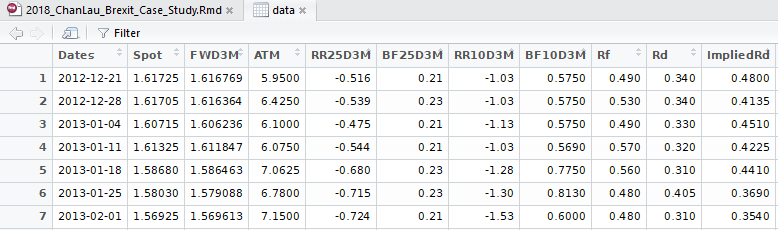
\includegraphics[width=1\linewidth]{images/figDataStructure} \end{center}

\end{frame}

\begin{frame}{The data (1)}

FX related

\begin{itemize}
\tightlist
\item
  Spot: the GBPUSD spot exchange rate, i.e.~USD per GBP
\item
  FWD3M: the 3-month GBPUSD forward exchange rate
\item
  Rf: the 3-month GBP money market deposit rate, annualized (in percent)
\item
  Rd: the 3-month USD money market deposit rate, annualized (in percent)
\end{itemize}

\end{frame}

\begin{frame}{The data (2)}

FX option related

\begin{itemize}
\tightlist
\item
  ATM: the at-the-money implied volatility of a GBPUSD option with
  strike price equal to ATM
\item
  RR25D3M: the price of a 25\(\Delta\) risk reversal, in annualized
  volatility units (in percent)
\item
  BF25D3M: the price of a 25\(\Delta\) butterfly spread, in annualized
  volatility units (in percent)
\item
  RR10D3M: the price of a 10\(\Delta\) risk reversal, in annualized
  volatility units (in percent)
\item
  BF10D3M: the price of a 10\(\Delta\) butterfly spread, in annualized
  volatility units (in percent)
\end{itemize}

\end{frame}

\begin{frame}{The data (3)}

\[ \text{Implied domestic rate from covered interest parity:  }F = S \frac{\exp \left(\text{Implied } R_d \times T\right)}{\exp \left(R_f \times T\right)} \]

\begin{center}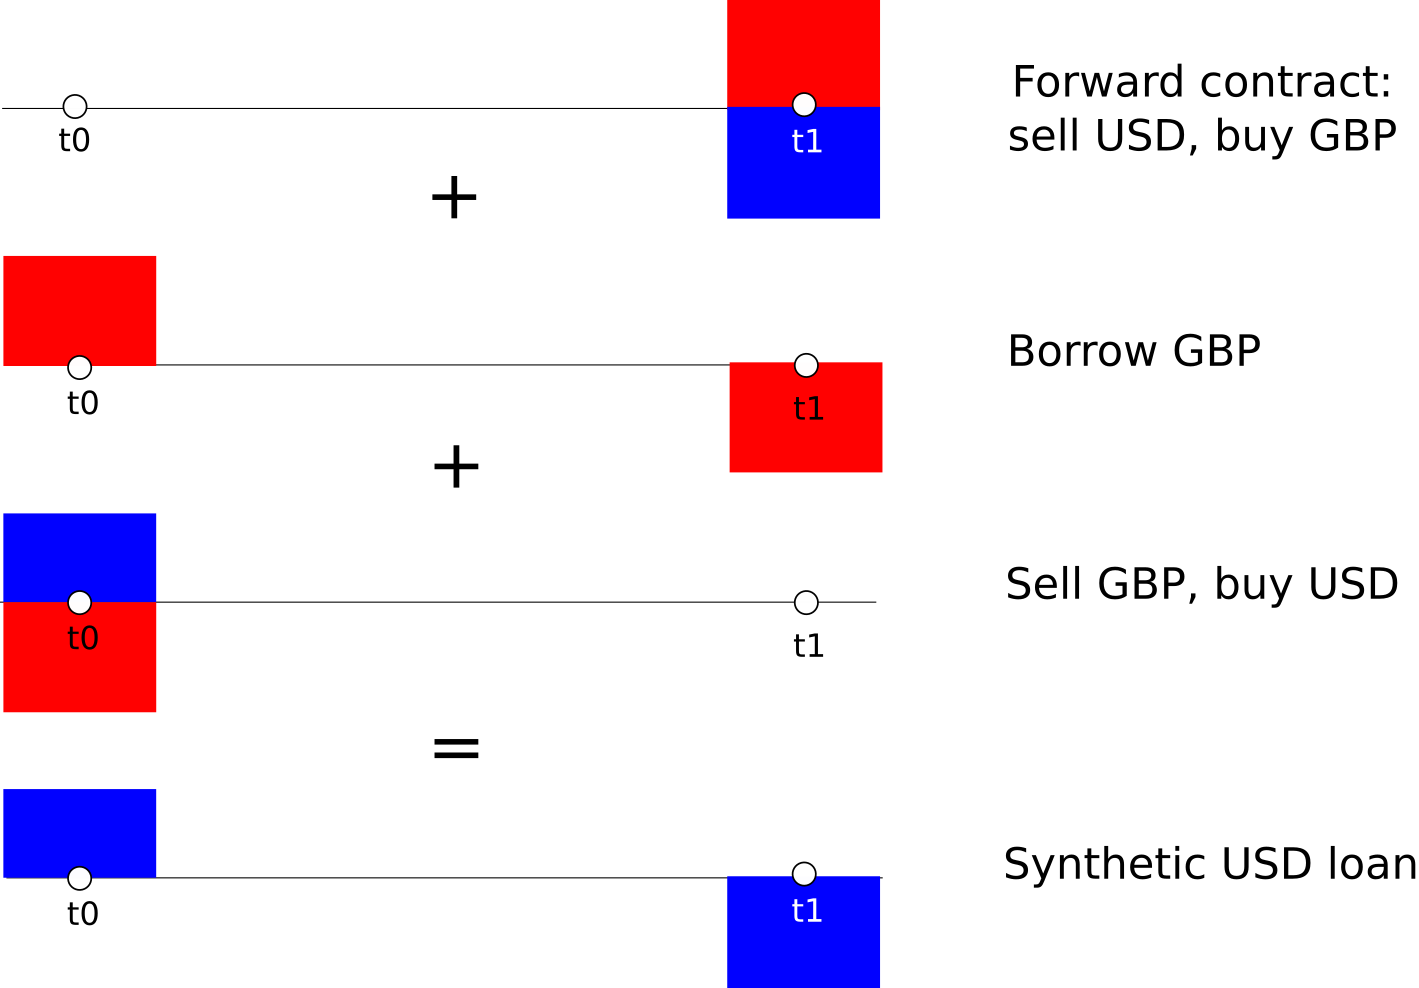
\includegraphics[width=0.6\linewidth]{images/figSyntheticUSDLoan} \end{center}

\end{frame}

\begin{frame}[fragile]{What the data tell us: spot and forward FX rates
(1)}

\begin{Shaded}
\begin{Highlighting}[]
\CommentTok{# Plot of the spot exchange rate with vertical line at Brexit vote}
\NormalTok{p1 =}\StringTok{ }\KeywordTok{ggplot}\NormalTok{(data, }\KeywordTok{aes}\NormalTok{(Dates, Spot)) }\OperatorTok{+}\StringTok{ }\KeywordTok{geom_line}\NormalTok{(}\DataTypeTok{colour=}\StringTok{"blue"}\NormalTok{) }
\NormalTok{p1 =}\StringTok{ }\NormalTok{p1 }\OperatorTok{+}\StringTok{ }\KeywordTok{geom_vline}\NormalTok{(}\DataTypeTok{xintercept=}\KeywordTok{as.POSIXct}\NormalTok{(}\KeywordTok{as.Date}\NormalTok{((}\StringTok{"2016-06-22 UTC"}\NormalTok{))),}
                     \DataTypeTok{linetype=}\StringTok{"longdash"}\NormalTok{)}
\NormalTok{p1}
\end{Highlighting}
\end{Shaded}

\begin{figure}
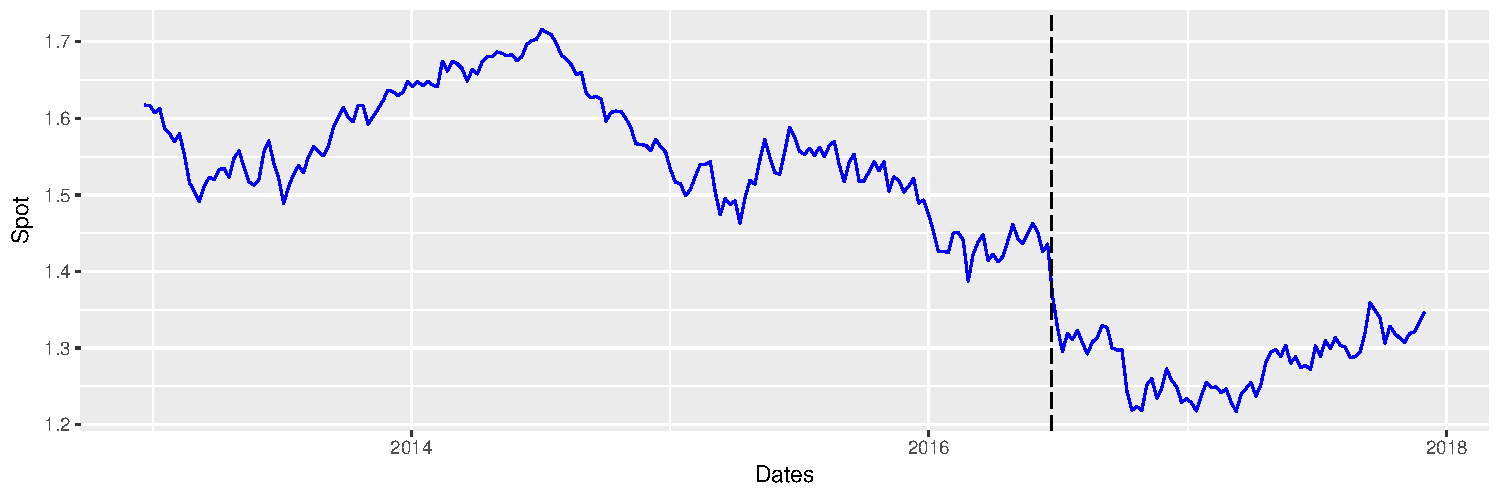
\includegraphics[width=1\linewidth]{2018_02_07_IMF_FXCourse_files/figure-beamer/unnamed-chunk-8-1} \caption{USDGBP spot exchange rate}\label{fig:unnamed-chunk-8}
\end{figure}

\end{frame}

\begin{frame}[fragile]{What the data tell us: spot and forward FX rates
(2)}

\begin{Shaded}
\begin{Highlighting}[]
\NormalTok{p2 =}\StringTok{ }\KeywordTok{ggplot}\NormalTok{(data, }\KeywordTok{aes}\NormalTok{(Dates, FWD3M)) }\OperatorTok{+}\StringTok{ }\KeywordTok{geom_line}\NormalTok{(}\DataTypeTok{colour=}\StringTok{"red"}\NormalTok{) }
\NormalTok{p2 =}\StringTok{ }\NormalTok{p2 }\OperatorTok{+}\StringTok{ }\KeywordTok{geom_vline}\NormalTok{(}\DataTypeTok{xintercept=}\KeywordTok{as.POSIXct}\NormalTok{(}\KeywordTok{as.Date}\NormalTok{((}\StringTok{"2016-06-22 UTC"}\NormalTok{))),}
                     \DataTypeTok{linetype=}\StringTok{"longdash"}\NormalTok{)}
\NormalTok{p2}
\end{Highlighting}
\end{Shaded}

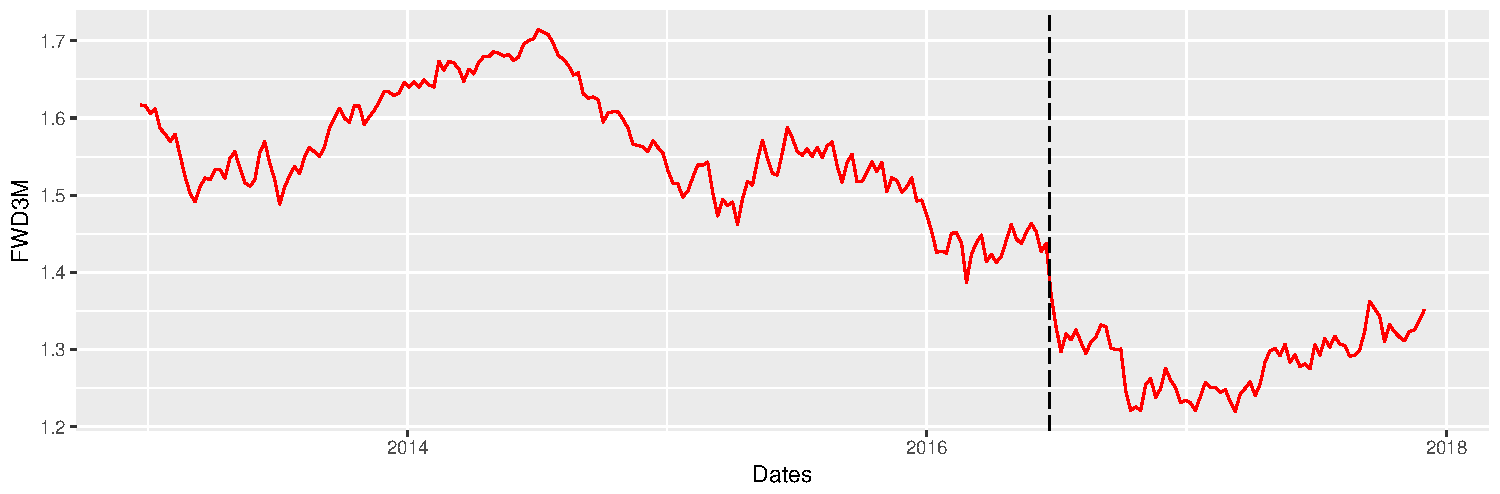
\includegraphics[width=1\linewidth]{2018_02_07_IMF_FXCourse_files/figure-beamer/unnamed-chunk-9-1}

\end{frame}

\begin{frame}[fragile]{What the data tell us: domestic rate
differentials}

\begin{Shaded}
\begin{Highlighting}[]
\NormalTok{data}\OperatorTok{$}\NormalTok{spreadRd =}\StringTok{ }\NormalTok{(data}\OperatorTok{$}\NormalTok{ImpliedRd }\OperatorTok{-}\StringTok{ }\NormalTok{data}\OperatorTok{$}\NormalTok{Rd)}\OperatorTok{*}\DecValTok{100}
\NormalTok{p3 =}\StringTok{ }\KeywordTok{ggplot}\NormalTok{(data, }\KeywordTok{aes}\NormalTok{(Dates, spreadRd)) }\OperatorTok{+}\StringTok{ }\KeywordTok{geom_line}\NormalTok{(}\DataTypeTok{colour=}\StringTok{"purple"}\NormalTok{) }\OperatorTok{+}\StringTok{ }
\StringTok{        }\KeywordTok{geom_hline}\NormalTok{(}\DataTypeTok{yintercept=}\DecValTok{0}\NormalTok{)}
\NormalTok{p3 =}\StringTok{ }\NormalTok{p3 }\OperatorTok{+}\StringTok{ }\KeywordTok{geom_vline}\NormalTok{(}\DataTypeTok{xintercept=}\KeywordTok{as.POSIXct}\NormalTok{(}\KeywordTok{as.Date}\NormalTok{((}\StringTok{"2016-06-22 UTC"}\NormalTok{))),}
                     \DataTypeTok{linetype=}\StringTok{"longdash"}\NormalTok{)}
\NormalTok{p3}
\end{Highlighting}
\end{Shaded}

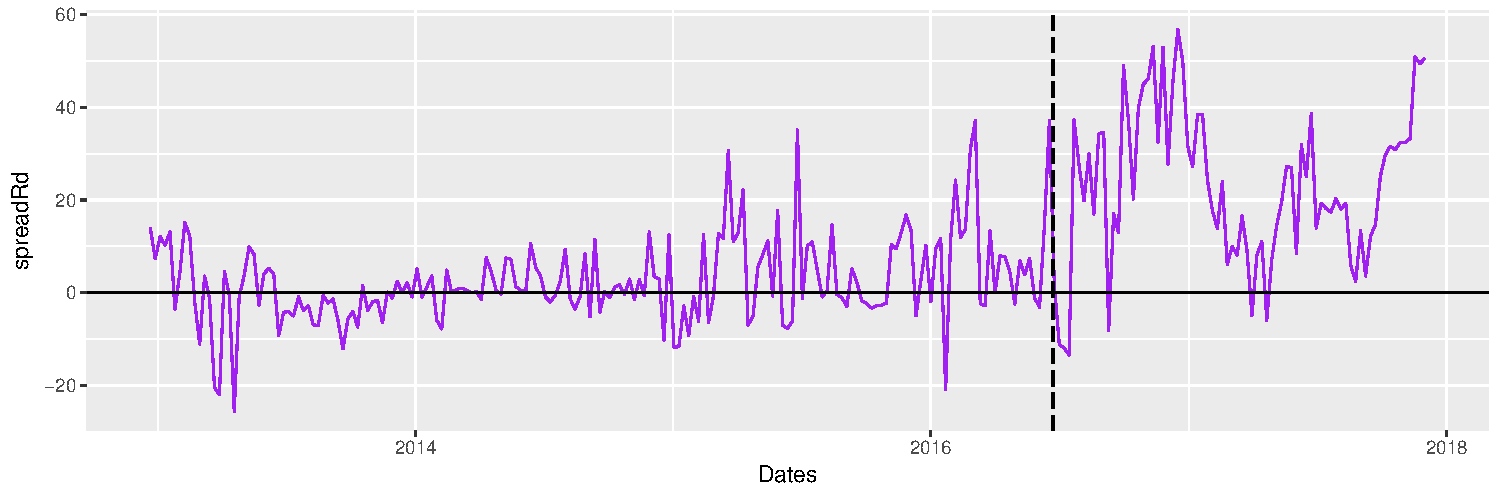
\includegraphics[width=1\linewidth]{2018_02_07_IMF_FXCourse_files/figure-beamer/unnamed-chunk-10-1}

\end{frame}

\begin{frame}[fragile]{What the data tell us: ATM volatility}

\begin{Shaded}
\begin{Highlighting}[]
\NormalTok{p4 =}\StringTok{ }\KeywordTok{ggplot}\NormalTok{(data, }\KeywordTok{aes}\NormalTok{(Dates, ATM)) }\OperatorTok{+}\StringTok{ }\KeywordTok{geom_line}\NormalTok{(}\DataTypeTok{colour=}\StringTok{"blue"}\NormalTok{) }\OperatorTok{+}\StringTok{ }
\StringTok{        }\KeywordTok{geom_hline}\NormalTok{(}\DataTypeTok{yintercept=}\DecValTok{0}\NormalTok{)}
\NormalTok{p4 =}\StringTok{ }\NormalTok{p4 }\OperatorTok{+}\StringTok{ }\KeywordTok{geom_vline}\NormalTok{(}\DataTypeTok{xintercept=}\KeywordTok{as.POSIXct}\NormalTok{(}\KeywordTok{as.Date}\NormalTok{((}\StringTok{"2016-06-22 UTC"}\NormalTok{))),}
                     \DataTypeTok{linetype=}\StringTok{"longdash"}\NormalTok{)}
\NormalTok{p4}
\end{Highlighting}
\end{Shaded}

\begin{figure}
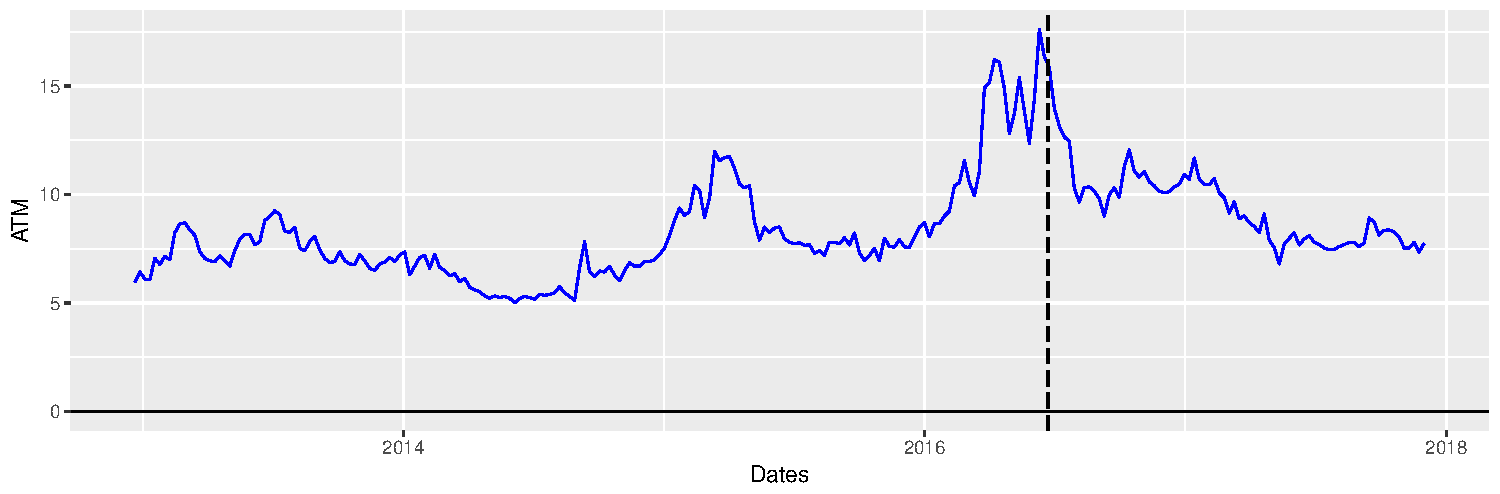
\includegraphics[width=1\linewidth]{2018_02_07_IMF_FXCourse_files/figure-beamer/unnamed-chunk-11-1} \caption{ATM volatility}\label{fig:unnamed-chunk-11}
\end{figure}

\end{frame}

\begin{frame}{What the data tell us: risk reversals (1)}

\begin{figure}
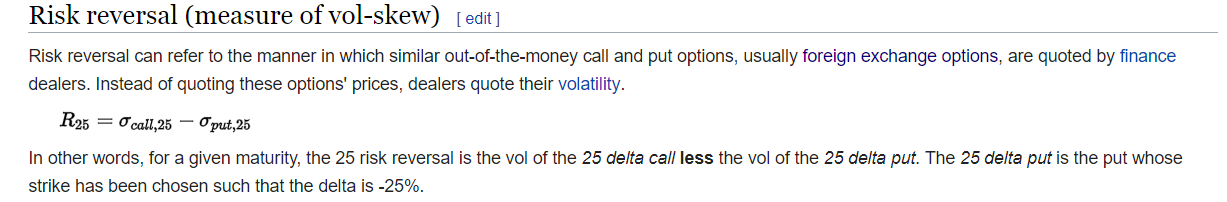
\includegraphics[width=1\linewidth]{images/figRRDefinition} \caption{Risk reversal definition (Wikipedia)}\label{fig:unnamed-chunk-12}
\end{figure}

\end{frame}

\begin{frame}{What the data tell us: risk reversals (2)}

\begin{itemize}
\tightlist
\item
  Full understanding of the risk reversal requires knowing what
  \(\Delta\) is
\item
  But without knowing, we still use risk reversal quotes to assess the
  prices market participants place on potential exchange rate movements.
\end{itemize}

\[
RR_{25\Delta} = \sigma_{25\Delta C} - \sigma_{25\Delta P}
\]

\begin{itemize}
\tightlist
\item
  Pay \(\sigma_{25\Delta C}\) for owning the call
\item
  Offset cost somewhat by selling the put at \(\sigma_{25\Delta P}\)
\end{itemize}

\end{frame}

\begin{frame}{What the data tell us: risk reversals (3)}

\begin{itemize}
\tightlist
\item
  Risk reversal payoff, long a call and short a put, both of them OTM:
\end{itemize}

\begin{figure}
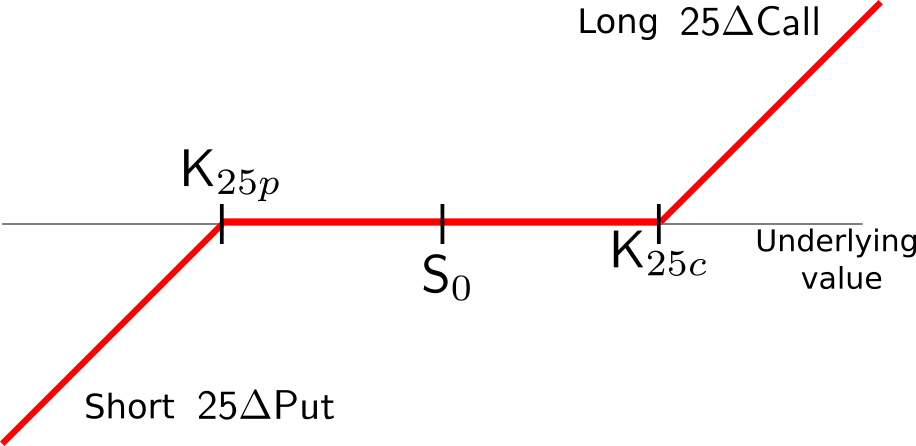
\includegraphics[width=0.7\linewidth]{images/fig25RRSimple} \caption{Risk reversal payoff at maturity}\label{fig:unnamed-chunk-13}
\end{figure}

\begin{itemize}
\tightlist
\item
  Explain why the price could be positive (or negative)?
\end{itemize}

\end{frame}

\begin{frame}[fragile]{What the data tell us: risk reversals (4)}

\begin{Shaded}
\begin{Highlighting}[]
\NormalTok{p5 =}\StringTok{ }\KeywordTok{ggplot}\NormalTok{(data, }\KeywordTok{aes}\NormalTok{(Dates, RR25D3M)) }\OperatorTok{+}\StringTok{ }\KeywordTok{geom_line}\NormalTok{(}\DataTypeTok{colour=}\StringTok{"red"}\NormalTok{) }\OperatorTok{+}\StringTok{ }
\StringTok{        }\KeywordTok{geom_hline}\NormalTok{(}\DataTypeTok{yintercept=}\DecValTok{0}\NormalTok{)}
\NormalTok{p5 =}\StringTok{ }\NormalTok{p5 }\OperatorTok{+}\StringTok{ }\KeywordTok{geom_vline}\NormalTok{(}\DataTypeTok{xintercept=}\KeywordTok{as.POSIXct}\NormalTok{(}\KeywordTok{as.Date}\NormalTok{((}\StringTok{"2016-06-22 UTC"}\NormalTok{))),}
                     \DataTypeTok{linetype=}\StringTok{"longdash"}\NormalTok{)}
\NormalTok{p5}
\end{Highlighting}
\end{Shaded}

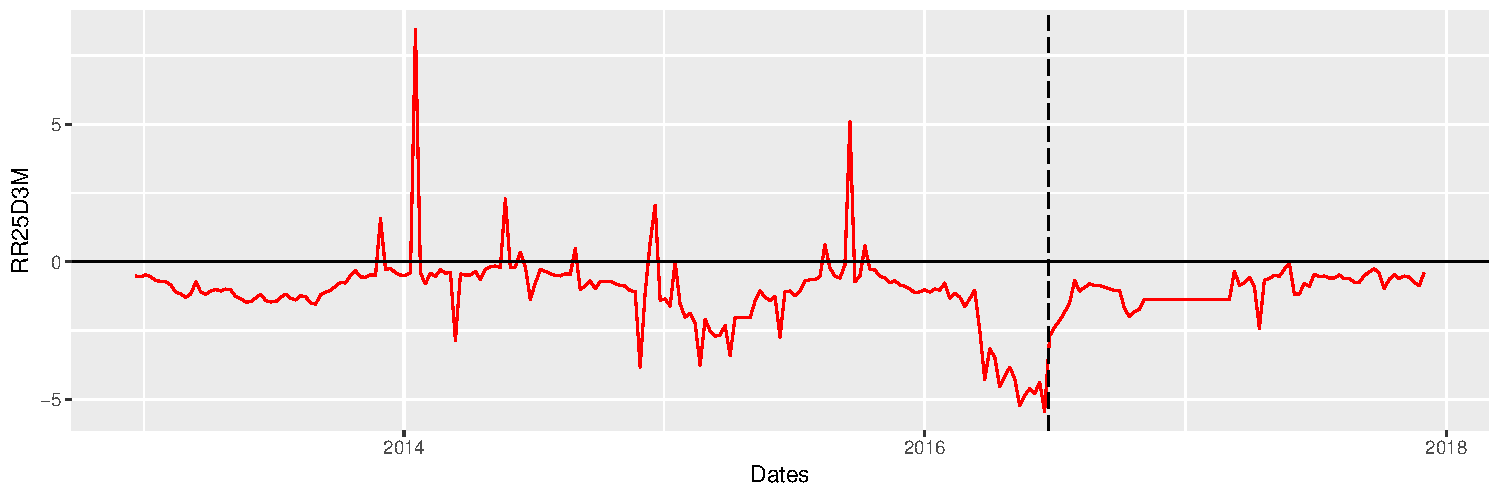
\includegraphics[width=1\linewidth]{2018_02_07_IMF_FXCourse_files/figure-beamer/unnamed-chunk-14-1}

\end{frame}

\begin{frame}[fragile]{What the data tell us: risk reversals (5)}

\begin{Shaded}
\begin{Highlighting}[]
\NormalTok{p6 =}\StringTok{ }\KeywordTok{ggplot}\NormalTok{(data, }\KeywordTok{aes}\NormalTok{(Dates, RR10D3M)) }\OperatorTok{+}\StringTok{ }\KeywordTok{geom_line}\NormalTok{(}\DataTypeTok{colour=}\StringTok{"blue"}\NormalTok{) }\OperatorTok{+}\StringTok{ }
\StringTok{        }\KeywordTok{geom_hline}\NormalTok{(}\DataTypeTok{yintercept=}\DecValTok{0}\NormalTok{)}
\NormalTok{p6 =}\StringTok{ }\NormalTok{p6 }\OperatorTok{+}\StringTok{ }\KeywordTok{geom_vline}\NormalTok{(}\DataTypeTok{xintercept=}\KeywordTok{as.POSIXct}\NormalTok{(}\KeywordTok{as.Date}\NormalTok{((}\StringTok{"2016-06-22 UTC"}\NormalTok{))),}
                     \DataTypeTok{linetype=}\StringTok{"longdash"}\NormalTok{)}
\NormalTok{p6}
\end{Highlighting}
\end{Shaded}

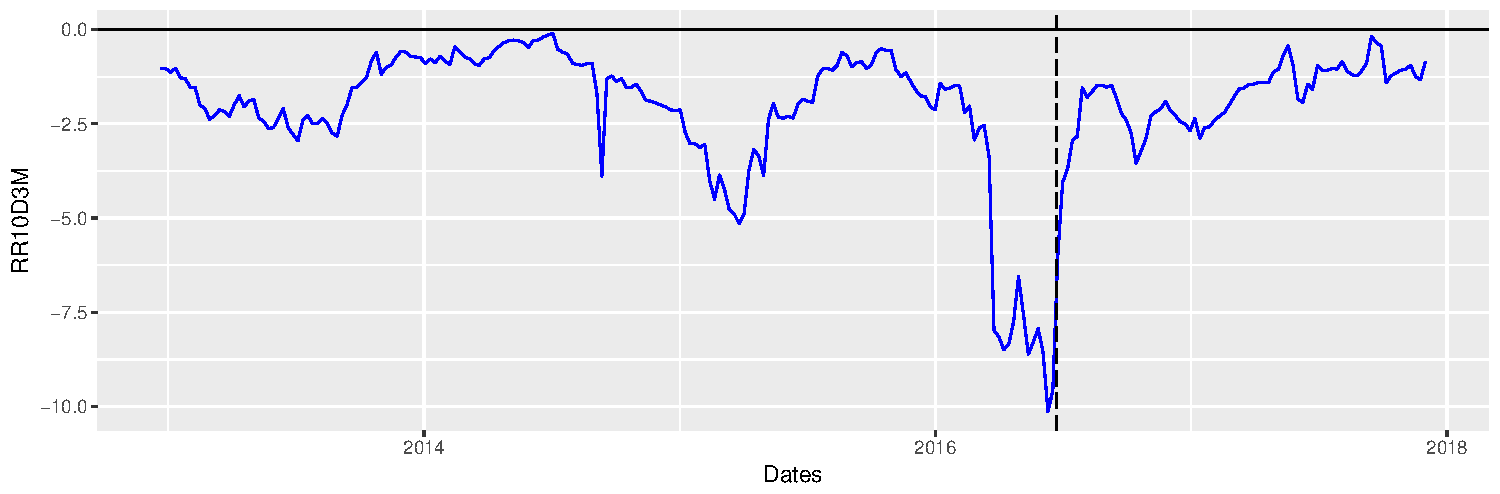
\includegraphics[width=1\linewidth]{2018_02_07_IMF_FXCourse_files/figure-beamer/unnamed-chunk-15-1}

\end{frame}

\begin{frame}{What the data tells us: butterfly spreads (1)}

\begin{itemize}
\tightlist
\item
  Suppose we want to profit from large movements of the exchange rate
\item
  The strangle would make our day !!
\end{itemize}

\begin{center}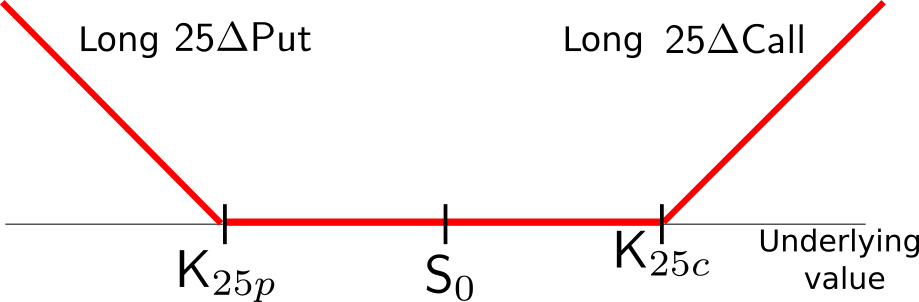
\includegraphics[width=0.7\linewidth]{images/fig25BFSimple} \end{center}

\end{frame}

\begin{frame}{What the data tells us: butterfly spreads (2)}

\begin{itemize}
\tightlist
\item
  The cost of the strangle is:
\end{itemize}

\[
S_{25\Delta} = \sigma_{25\Delta C} + \sigma_{25\Delta P}
\]

\begin{itemize}
\tightlist
\item
  But markets don't quote strangles\\[2\baselineskip]
\item
  They quote \textbf{Butterfly Spreads}
\end{itemize}

\[
BF_{25\Delta} = \frac{\sigma_{25\Delta C} + \sigma_{25\Delta P}}{2}  - \sigma_{ATM}
\]

\end{frame}

\begin{frame}{What the data tells us: butterfly spreads (3)}

\begin{itemize}
\tightlist
\item
  Butterfly spreads convey more information
\end{itemize}

\begin{center}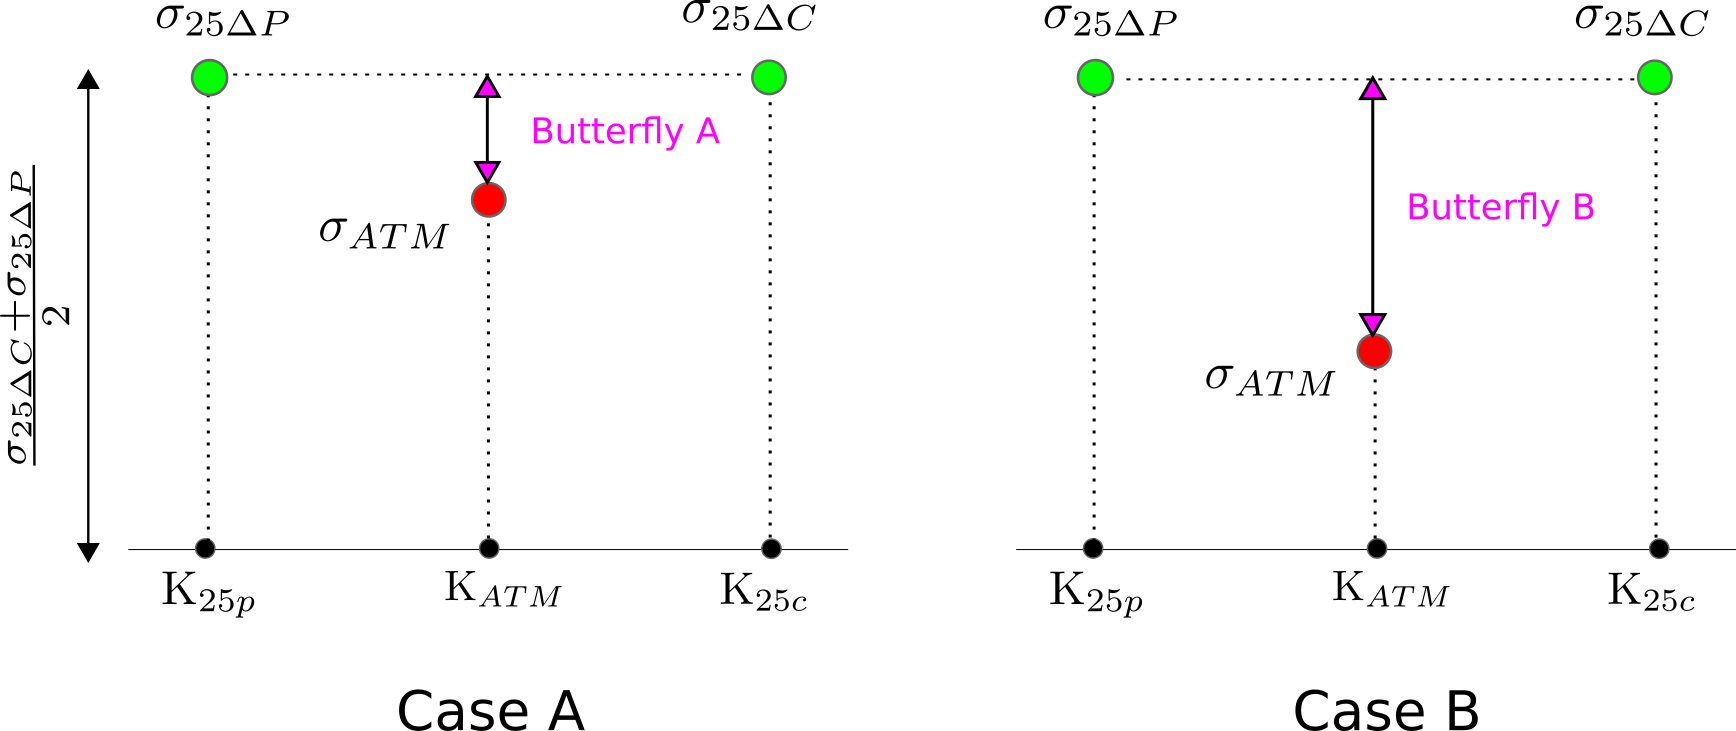
\includegraphics[width=1\linewidth]{images/figStrangleButterfly} \end{center}

\end{frame}

\begin{frame}[fragile]{What the data tells us: butterfly spreads (4)}

\begin{Shaded}
\begin{Highlighting}[]
\NormalTok{p7 =}\StringTok{ }\KeywordTok{ggplot}\NormalTok{(data, }\KeywordTok{aes}\NormalTok{(Dates, BF25D3M)) }\OperatorTok{+}\StringTok{ }\KeywordTok{geom_line}\NormalTok{(}\DataTypeTok{colour=}\StringTok{"red"}\NormalTok{) }\OperatorTok{+}\StringTok{ }
\StringTok{        }\KeywordTok{geom_hline}\NormalTok{(}\DataTypeTok{yintercept=}\DecValTok{0}\NormalTok{)}
\NormalTok{p7 =}\StringTok{ }\NormalTok{p7 }\OperatorTok{+}\StringTok{ }\KeywordTok{geom_vline}\NormalTok{(}\DataTypeTok{xintercept=}\KeywordTok{as.POSIXct}\NormalTok{(}\KeywordTok{as.Date}\NormalTok{((}\StringTok{"2016-06-22 UTC"}\NormalTok{))),}
                     \DataTypeTok{linetype=}\StringTok{"longdash"}\NormalTok{)}
\NormalTok{p7}
\end{Highlighting}
\end{Shaded}

\begin{center}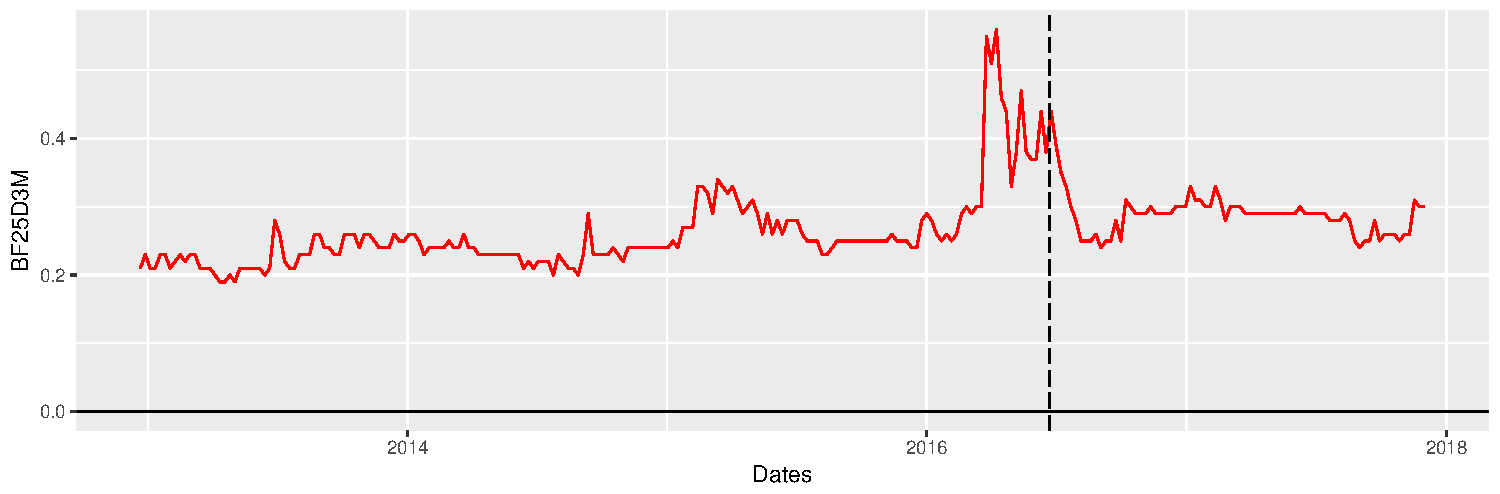
\includegraphics[width=1\linewidth]{2018_02_07_IMF_FXCourse_files/figure-beamer/unnamed-chunk-18-1} \end{center}

\end{frame}

\begin{frame}[fragile]{What the data tells us: butterfly spreads (5)}

\begin{Shaded}
\begin{Highlighting}[]
\NormalTok{p8 =}\StringTok{ }\KeywordTok{ggplot}\NormalTok{(data, }\KeywordTok{aes}\NormalTok{(Dates, BF10D3M)) }\OperatorTok{+}\StringTok{ }\KeywordTok{geom_line}\NormalTok{(}\DataTypeTok{colour=}\StringTok{"blue"}\NormalTok{) }\OperatorTok{+}\StringTok{ }
\StringTok{        }\KeywordTok{geom_hline}\NormalTok{(}\DataTypeTok{yintercept=}\DecValTok{0}\NormalTok{)}
\NormalTok{p8 =}\StringTok{ }\NormalTok{p8 }\OperatorTok{+}\StringTok{ }\KeywordTok{geom_vline}\NormalTok{(}\DataTypeTok{xintercept=}\KeywordTok{as.POSIXct}\NormalTok{(}\KeywordTok{as.Date}\NormalTok{((}\StringTok{"2016-06-22 UTC"}\NormalTok{))),}
                     \DataTypeTok{linetype=}\StringTok{"longdash"}\NormalTok{)}
\NormalTok{p8}
\end{Highlighting}
\end{Shaded}

\begin{center}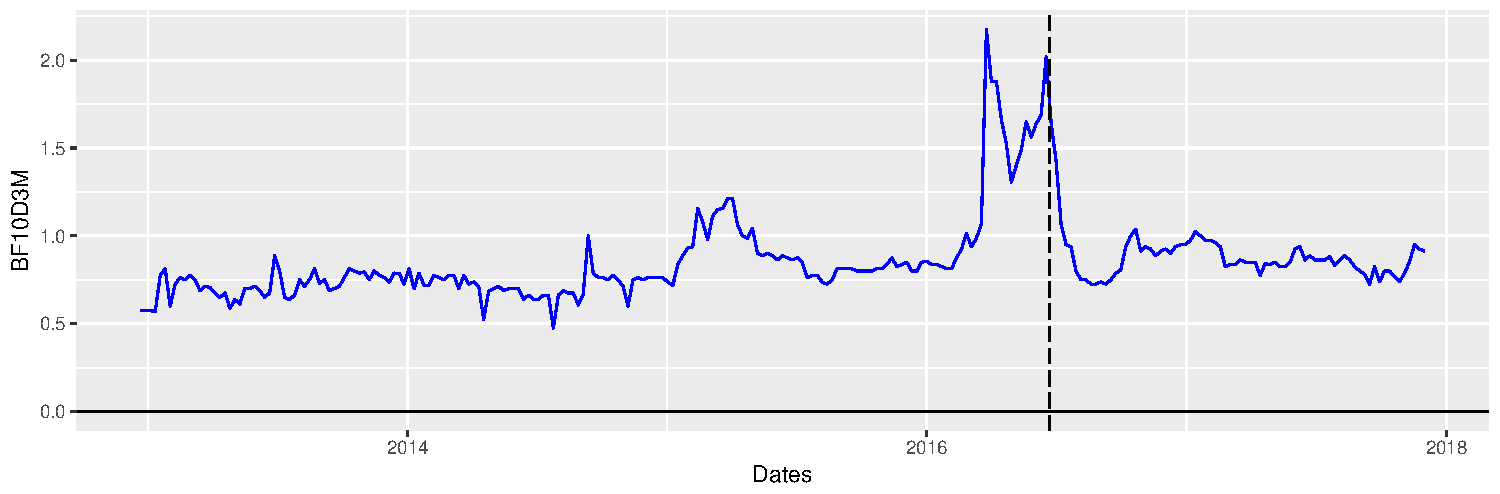
\includegraphics[width=1\linewidth]{2018_02_07_IMF_FXCourse_files/figure-beamer/unnamed-chunk-19-1} \end{center}

\end{frame}

\begin{frame}{}

\color{blue} \LARGE{Part C:}\\
\LARGE{A Little Bit of Option Pricing}

\end{frame}

\begin{frame}{What is \(\Delta\) (1)}

\begin{itemize}
\tightlist
\item
  The \(\Delta\) of a call
\end{itemize}

\[ \Delta_C = \frac{\partial C}{\partial S} \geq 0\]

\begin{itemize}
\tightlist
\item
  The \(\Delta\) of a put
\end{itemize}

\[ \Delta_P = \frac{\partial P}{\partial S} \leq 0\]

\end{frame}

\begin{frame}{What is \(\Delta\) (2)}

\begin{center}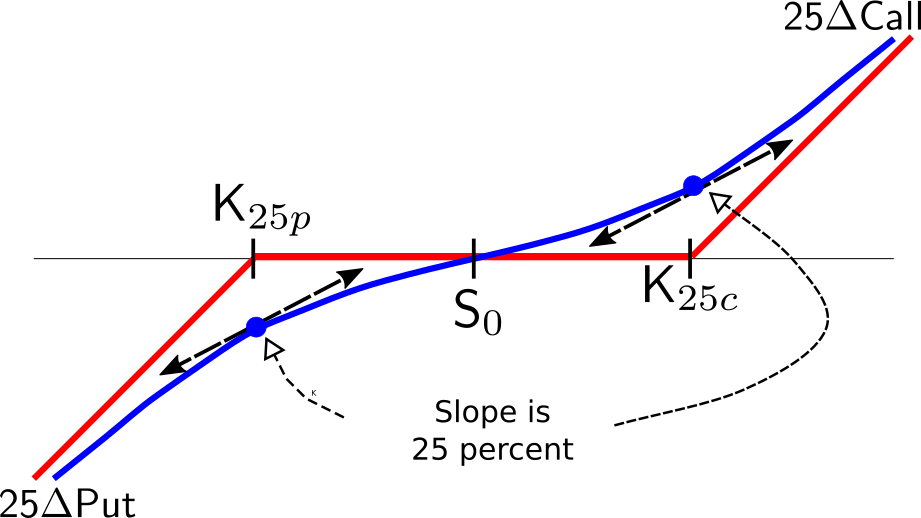
\includegraphics[width=0.8\linewidth]{images/fig25RR} \end{center}

\end{frame}

\begin{frame}{What is \(\Delta\) (3)}

\begin{center}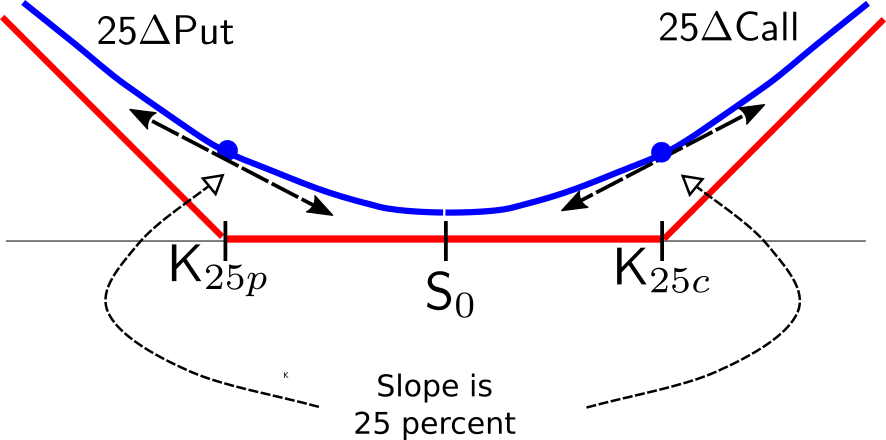
\includegraphics[width=0.8\linewidth]{images/fig25Strangle} \end{center}

\end{frame}

\begin{frame}{What is \(\Delta\) (4)}

\begin{center}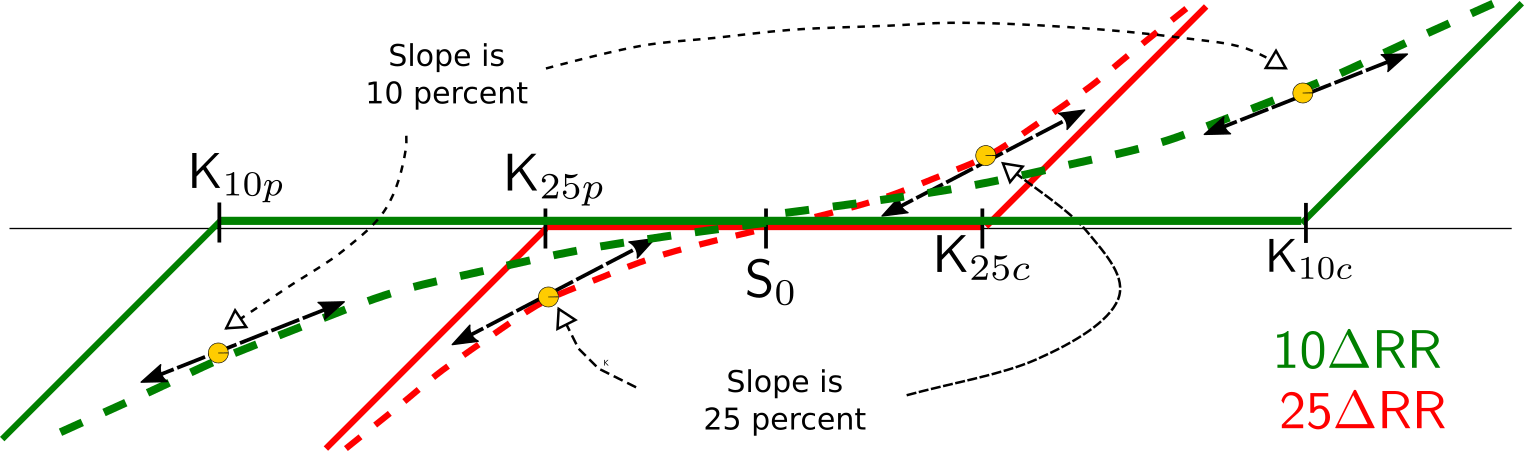
\includegraphics[width=1\linewidth]{images/fig1025RR} \end{center}

\end{frame}

\begin{frame}{Option prices = replication cost (1)}

Dealer costs when buying call option from client

\begin{itemize}
\tightlist
\item
  Funding cost: borrow \(C\) at \(R_d\): \(R_d C_t \delta t\)\\
\item
  Hedging cost (using delta-hedging)

  \begin{itemize}
  \tightlist
  \item
    Borrow and sell \(\Delta\) units of foreign currency
  \item
    Receive \(\Delta S\) and reinvest at \(R_d\)
  \item
    Pay accrued interest on borrowed amount of currency
  \item
    Net gain: \((R_d - R_f)\Delta S_t \delta t\)
  \end{itemize}
\end{itemize}

\end{frame}

\begin{frame}{Option price = replication cost (2)}

\begin{itemize}
\tightlist
\item
  Time decay of option: loses value as maturity approaches
  \[\frac{\partial C_t}{\partial t} \delta t\]\\
  \hspace*{0.333em}
\item
  Convexity gains since options are non-linear
  \[ \frac{\partial^2 C_t}{\partial S^2}(\delta S_t)^2\]
\end{itemize}

\end{frame}

\begin{frame}{Option price = replication cost (3)}

\begin{itemize}
\tightlist
\item
  Gains must offset costs, yielding the pricing partial differential
  equation:
\end{itemize}

\[
\frac{\partial C_t}{\partial t} \delta t + (R_d - R_f) \Delta S_t  \delta t + \frac{\partial^2 C}{\partial S_t^2} (\delta S_t)^2 = R_d C_t \delta t
\]

\end{frame}

\begin{frame}{Garman-Kohlhagen formula (1)}

Assume FX follows a geometric brownian motion, the call option price is:

\[
\boxed{
C(K,S_t,R_d,R_f,T,\sigma) = S_t \exp(-R_f\times(T-t))N(d_1) - K\exp(-R_d \times (T-t))N(d_2)
}
\]

and the put option price is:

\[
\boxed{
P(K,S_t,R_d,R_f,T,\sigma) = K\exp(-R_d \times (T-t))N(-d_2) - S_t \exp(-R_f\times(T-t))N(-d_1) 
}
\]

\end{frame}

\begin{frame}{Garman-Kohlhagen formula (2)}

\begin{itemize}
\tightlist
\item
  \(K\) is the strike price,
\item
  \(S_t\) is the current spot exchange rate,
\item
  \(R_d\) is the domestic interest rate,
\item
  \(R_f\) is the foreign interest rate,
\item
  \(T-t\) is the remaining life of an option maturing at time \(T\),
\item
  \(\sigma\) is the implied volatility of the exchange rate used to
  price the option,
\item
  \[
  \begin{aligned}
  d_1 &= \frac{\ln(S_t/K)+(R_d-R_f+\sigma^2/2)(T-t)}{\sigma \times (T-t)}\\
  d_2 &= d_1 - \sigma \times (T-t)
  \end{aligned}
  \]
\end{itemize}

\end{frame}

\begin{frame}{Implied volatility \(\sigma\) (1)}

\begin{itemize}
\tightlist
\item
  All GK formula inputs are observable except implied volatility
  \(\sigma\)\\[2\baselineskip]
\item
  Option prices are quoted as \textbf{vols},
  i.e.~volatility\\[2\baselineskip]
\item
  To obtain price

  \begin{itemize}
  \tightlist
  \item
    Take quoted vol
  \item
    Use reference values for all other variables
  \item
    Plug into GK formula
  \end{itemize}
\end{itemize}

\end{frame}

\begin{frame}{Implied volatility \(\sigma\) (2)}

Implied volatility

\begin{itemize}
\tightlist
\item
  is different from historical or realized volatility\\[2\baselineskip]
\item
  is not a forecast of future volatility\\[2\baselineskip]
\item
  yields an GK option premium reflecting

  \begin{itemize}
  \tightlist
  \item
    profit margin
  \item
    hedging costs
  \item
    demand and supply in the FX market
  \end{itemize}
\end{itemize}

\end{frame}

\begin{frame}{}

\color{blue} \LARGE{Part D:}\\
\LARGE{The Volatility Smile}

\end{frame}

\begin{frame}{Finding vols for different \(\Delta\)s}

\begin{itemize}
\item
  For a given \(\Delta\) we have prices for:

  \begin{itemize}
  \tightlist
  \item
    Risk reversal (RR)
  \item
    Butterfly spread (BF)
  \end{itemize}
\item
  The ATM vol, \(\sigma_{ATM}\) is also given
\item
  From the definitions of the RR and the BF
\end{itemize}

\[
\begin{aligned}
  \sigma_{25\Delta C} &= \sigma_{ATM} + BF_{25\Delta} + \frac{1}{2} RR_{25\Delta}\\
  \sigma_{25\Delta P} &= \sigma_{ATM} + BF_{25\Delta} - \frac{1}{2} RR_{25\Delta}\\
  \sigma_{75\Delta C} &= \sigma_{25\Delta P}\enspace \text{by put-call parity}
\end{aligned}
\]

\begin{itemize}
\tightlist
\item
  Plotting \(\sigma\) against \(\Delta\) yields the volatility smile
\end{itemize}

\end{frame}

\begin{frame}{The level of the smile: \(\sigma_{ATM}\)}

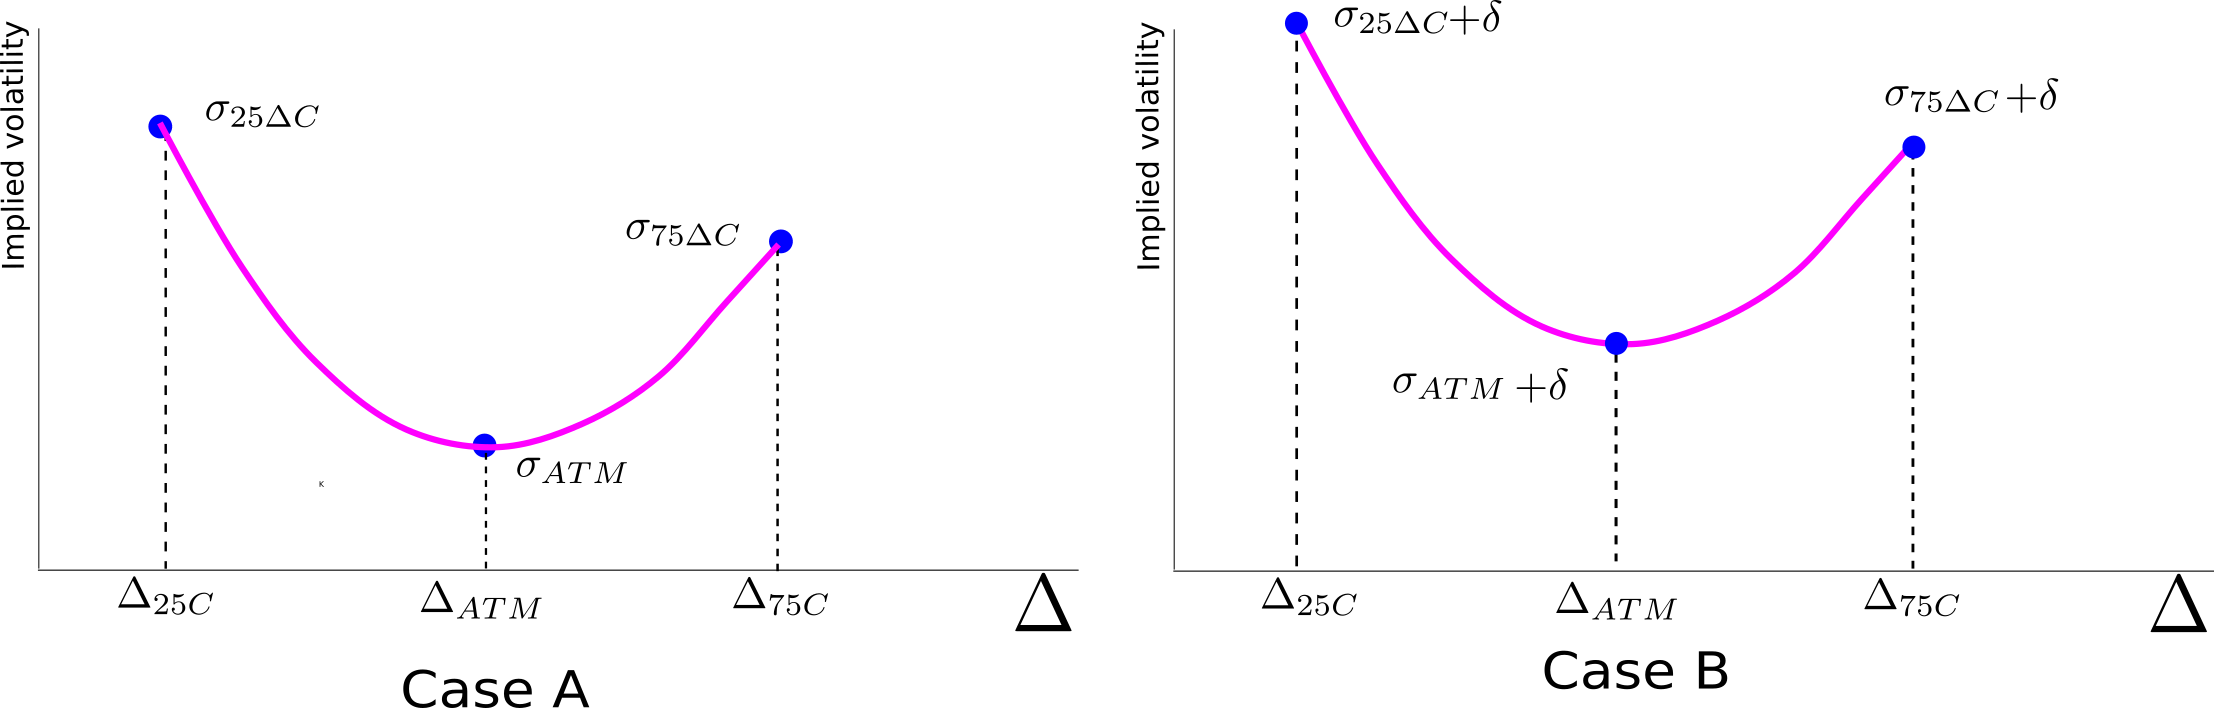
\includegraphics[width=1\linewidth]{images/figRRLevel}

\end{frame}

\begin{frame}{The slope of the smile: the risk reversal}

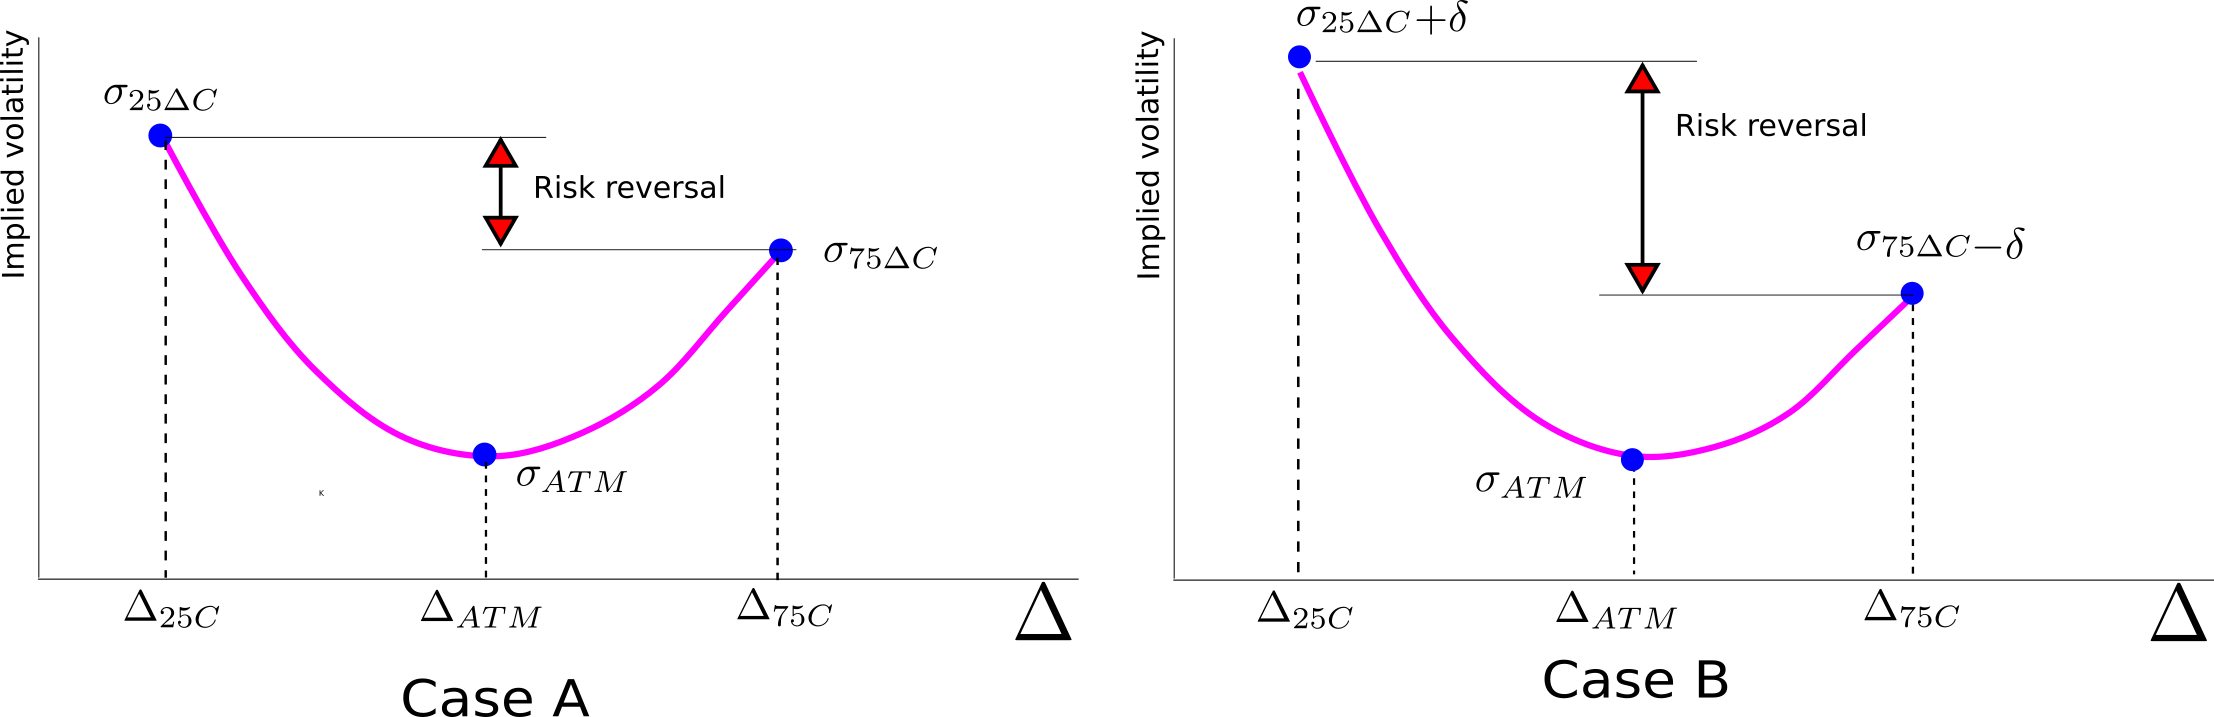
\includegraphics[width=1\linewidth]{images/figRRSlope}

\end{frame}

\begin{frame}{The slope of the smile: the butterfly spread}

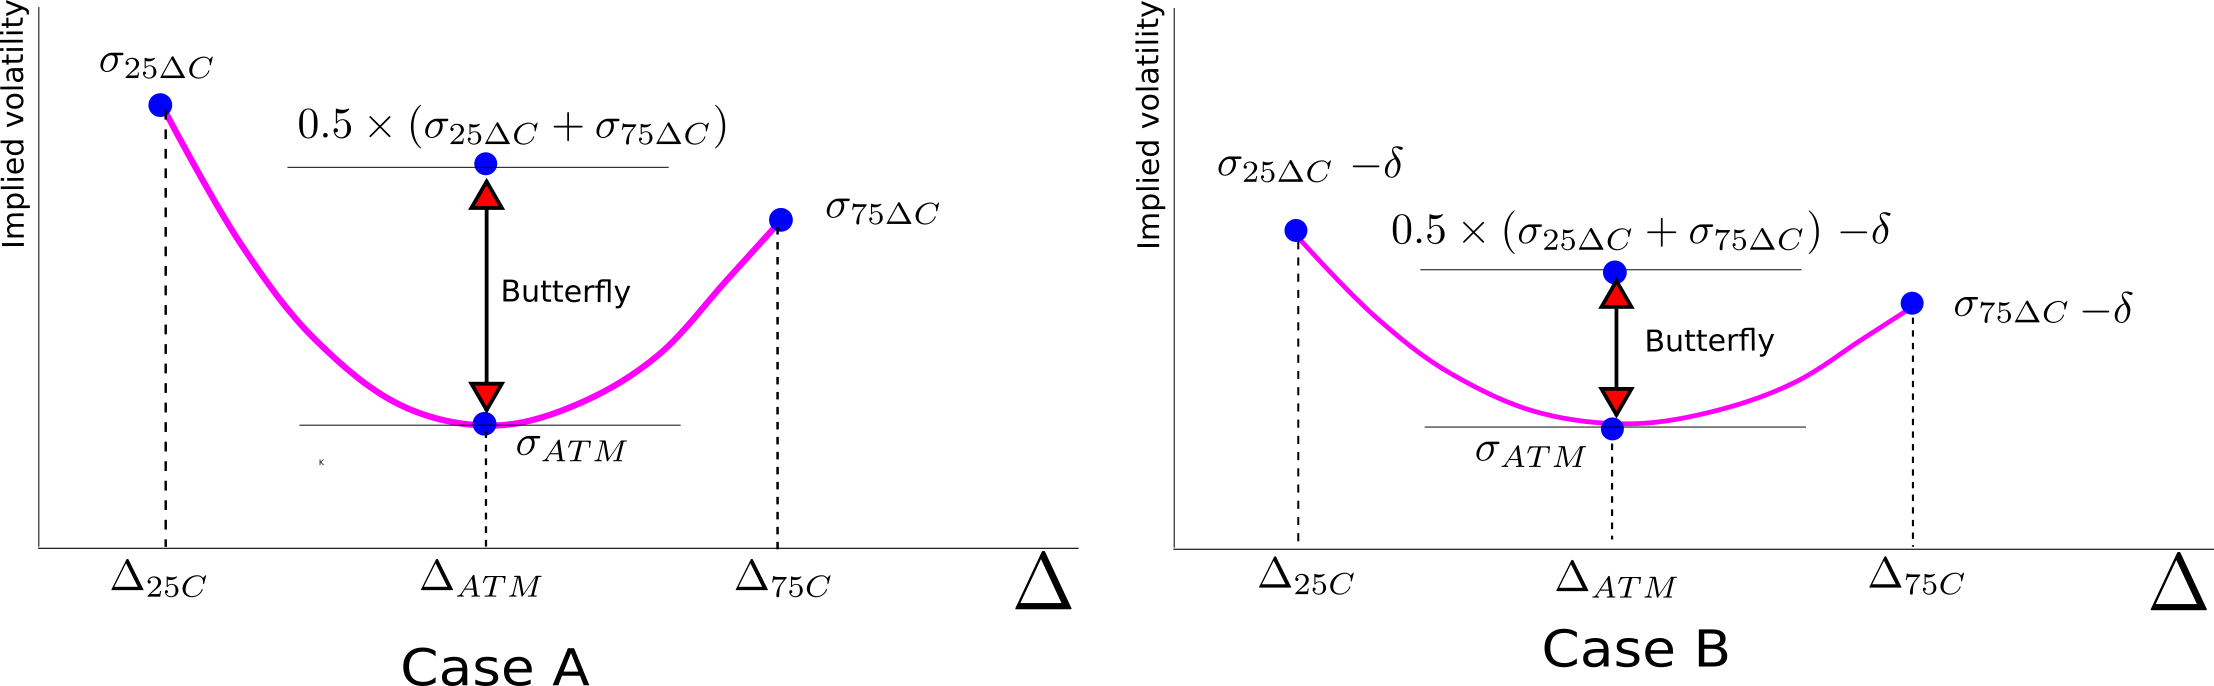
\includegraphics[width=1\linewidth]{images/figRRCurvature}

\end{frame}

\begin{frame}{}

\color{blue} \LARGE{Part E:}\\
\LARGE{Constructing the Volatility Smile: Brexit}

\end{frame}

\begin{frame}{Selecting the dates}

We are interested in the behavior of the GBPUSD for three dates:

\begin{itemize}
\tightlist
\item
  January 8, 2016 (Pre-Brexit)
\item
  June 24, 2016 (Brexit)
\item
  December 1, 2017 (Post-Brexit)
\end{itemize}

\end{frame}

\begin{frame}[fragile]{Getting the data (1)}

\begin{Shaded}
\begin{Highlighting}[]
\KeywordTok{rm}\NormalTok{(}\DataTypeTok{list=}\KeywordTok{ls}\NormalTok{())                                     }\CommentTok{# Clean up memory}
\NormalTok{filename =}\StringTok{ "2018_IET_Options_data.csv"}            \CommentTok{# Name of CSV data file}
\NormalTok{data =}\StringTok{ }\KeywordTok{read.csv}\NormalTok{(filename, }\DataTypeTok{header=}\OtherTok{TRUE}\NormalTok{)            }\CommentTok{# Load datafile}
\NormalTok{data}\OperatorTok{$}\NormalTok{Dates =}\StringTok{ }\KeywordTok{mdy_hm}\NormalTok{(}\KeywordTok{as.character}\NormalTok{(data}\OperatorTok{$}\NormalTok{Dates))     }\CommentTok{# convert dates to Date class}
\KeywordTok{rownames}\NormalTok{(data)=}\OtherTok{NULL}                               \CommentTok{# remove row names}

\CommentTok{# Specify dates for analysis}

\NormalTok{date01 =}\StringTok{ }\KeywordTok{as.Date}\NormalTok{(}\StringTok{"2016-01-08 UTC"}\NormalTok{)                 }
\NormalTok{date02 =}\StringTok{ }\KeywordTok{as.Date}\NormalTok{(}\StringTok{"2016-06-24 UTC"}\NormalTok{)}
\NormalTok{date03 =}\StringTok{ }\KeywordTok{as.Date}\NormalTok{(}\StringTok{"2016-12-30 UTC"}\NormalTok{)}
\end{Highlighting}
\end{Shaded}

\end{frame}

\begin{frame}[fragile]{Getting the data (2)}

\begin{Shaded}
\begin{Highlighting}[]
\CommentTok{# Create data frame this.data}

\NormalTok{this.data =}\StringTok{ }\KeywordTok{rbind}\NormalTok{(}
\NormalTok{  data[}\KeywordTok{which}\NormalTok{(data}\OperatorTok{$}\NormalTok{Dates}\OperatorTok{==}\NormalTok{date01),],}
\NormalTok{  data[}\KeywordTok{which}\NormalTok{(data}\OperatorTok{$}\NormalTok{Dates}\OperatorTok{==}\NormalTok{date02),],}
\NormalTok{  data[}\KeywordTok{which}\NormalTok{(data}\OperatorTok{$}\NormalTok{Dates}\OperatorTok{==}\NormalTok{date03),])}

\CommentTok{# Delete row names and change the names of the columns}

\KeywordTok{rownames}\NormalTok{(this.data) =}\StringTok{ }\OtherTok{NULL}
\KeywordTok{colnames}\NormalTok{(this.data) =}\StringTok{ }\KeywordTok{c}\NormalTok{(}\StringTok{"Date"}\NormalTok{,}\StringTok{"spot"}\NormalTok{,}\StringTok{"forward"}\NormalTok{,}\StringTok{"atm"}\NormalTok{, }\StringTok{"rr25"}\NormalTok{,}\StringTok{"bf25"}\NormalTok{,}
                        \StringTok{"rr10"}\NormalTok{,}\StringTok{"bf10"}\NormalTok{,}\StringTok{"rf"}\NormalTok{,}\StringTok{"rd"}\NormalTok{,}\StringTok{"imp_rd"}\NormalTok{)}
\end{Highlighting}
\end{Shaded}

\end{frame}

\begin{frame}{Get additional vols}

In addition to the 25\(\Delta\) and 75\(\Delta\) vols, obtain the
10\(\Delta\) and 90\(\Delta\) vols:

\[
\begin{aligned}
  \sigma_{10\Delta C} &= \sigma_{ATM} + BF_{10\Delta} + \frac{1}{2} RR_{10\Delta}\\
  \sigma_{10\Delta P} &= \sigma_{ATM} + BF_{10\Delta} - \frac{1}{2} RR_{10\Delta}\\
  \sigma_{90\Delta C} &= \sigma_{10\Delta P}
\end{aligned}
\]

\end{frame}

\begin{frame}[fragile]{Calculating the implied vols (1)}

\begin{Shaded}
\begin{Highlighting}[]
\CommentTok{# Vols are in percent, expressed them as simple numbers}
\NormalTok{this.data}\OperatorTok{$}\NormalTok{atm  =}\StringTok{ }\NormalTok{this.data}\OperatorTok{$}\NormalTok{atm}\OperatorTok{/}\DecValTok{100}
\NormalTok{this.data}\OperatorTok{$}\NormalTok{rr25 =}\StringTok{ }\NormalTok{this.data}\OperatorTok{$}\NormalTok{rr25}\OperatorTok{/}\DecValTok{100}
\NormalTok{this.data}\OperatorTok{$}\NormalTok{bf25 =}\StringTok{ }\NormalTok{this.data}\OperatorTok{$}\NormalTok{bf25}\OperatorTok{/}\DecValTok{100}
\NormalTok{this.data}\OperatorTok{$}\NormalTok{rr10 =}\StringTok{ }\NormalTok{this.data}\OperatorTok{$}\NormalTok{rr10}\OperatorTok{/}\DecValTok{100}
\NormalTok{this.data}\OperatorTok{$}\NormalTok{bf10 =}\StringTok{ }\NormalTok{this.data}\OperatorTok{$}\NormalTok{bf10}\OperatorTok{/}\DecValTok{100}
\NormalTok{this.data}\OperatorTok{$}\NormalTok{rf   =}\StringTok{ }\NormalTok{this.data}\OperatorTok{$}\NormalTok{rf}\OperatorTok{/}\DecValTok{100}
\NormalTok{this.data}\OperatorTok{$}\NormalTok{rd   =}\StringTok{ }\NormalTok{this.data}\OperatorTok{$}\NormalTok{rd}\OperatorTok{/}\DecValTok{100}
\NormalTok{this.data}\OperatorTok{$}\NormalTok{imp_rd=this.data}\OperatorTok{$}\NormalTok{imp_rd}\OperatorTok{/}\DecValTok{100}

\CommentTok{# We will use this.data repeatedly}
\CommentTok{# Attach it to access its elements}

\KeywordTok{attach}\NormalTok{(this.data)     }
\end{Highlighting}
\end{Shaded}

\end{frame}

\begin{frame}[fragile]{Calculating the implied vols (2)}

\begin{Shaded}
\begin{Highlighting}[]
\CommentTok{# Recover vols for different deltas and put them in the data frame}

\NormalTok{this.data}\OperatorTok{$}\NormalTok{sigma10c =}\StringTok{ }\NormalTok{atm }\OperatorTok{+}\StringTok{ }\NormalTok{bf10 }\OperatorTok{+}\StringTok{ }\FloatTok{0.5}\OperatorTok{*}\NormalTok{rr10}
\NormalTok{this.data}\OperatorTok{$}\NormalTok{sigma25c =}\StringTok{ }\NormalTok{atm }\OperatorTok{+}\StringTok{ }\NormalTok{bf25 }\OperatorTok{+}\StringTok{ }\FloatTok{0.5}\OperatorTok{*}\NormalTok{rr25}
\NormalTok{this.data}\OperatorTok{$}\NormalTok{sigma75c =}\StringTok{ }\NormalTok{this.data}\OperatorTok{$}\NormalTok{sigma25c }\OperatorTok{-}\StringTok{ }\NormalTok{rr25}
\NormalTok{this.data}\OperatorTok{$}\NormalTok{sigma90c =}\StringTok{ }\NormalTok{this.data}\OperatorTok{$}\NormalTok{sigma10c }\OperatorTok{-}\StringTok{ }\NormalTok{rr10}
\NormalTok{this.data}\OperatorTok{$}\NormalTok{sigmaatm =}\StringTok{ }\NormalTok{atm}

\NormalTok{Tenor =}\StringTok{ }\DecValTok{3}\OperatorTok{/}\DecValTok{12}   \CommentTok{# Maturity of options, 3 months, in years}
\end{Highlighting}
\end{Shaded}

\end{frame}

\begin{frame}{What is the \(ATM\) strike?}

\begin{itemize}
\tightlist
\item
  Retail products \[
  \begin{aligned}
  K_{ATM} &= S\\
  \Delta_{ATM} &= N \left(\frac{\log(F/S) + \frac{1}{2} \sigma_{ATM}^2 T}{\sigma_{ATM} \sqrt T} \right)
  \end{aligned}
  \]
\item
  EM currencies, maturities more than one year \[
  \begin{aligned}
  K_{ATM} &= F\\
  \Delta_{ATM} &= \exp(-Rf \times T)N(\frac{1}{2}\sigma_{ATM} \sqrt T) 
  \end{aligned}
  \]
\item
  Major currencies, maturities of one year or less \[
  \begin{aligned}
   K_{ATM} &= F \times \exp\left( 0.5 \sigma^2_{ATM}\times T \right)\\
   \Delta_{ATM} &= 0.5\times exp(-Rf \times T) \simeq 0.5 
  \end{aligned}
  \]
\end{itemize}

\end{frame}

\begin{frame}[fragile]{Calculate the \(\Delta_{ATM}\)}

\begin{Shaded}
\begin{Highlighting}[]
\CommentTok{# Calculate the strike of the ATM option}
\NormalTok{K_atm =}\StringTok{ }\NormalTok{forward}\OperatorTok{*}\KeywordTok{exp}\NormalTok{((}\FloatTok{0.5}\OperatorTok{*}\NormalTok{(this.data}\OperatorTok{$}\NormalTok{sigmaatm)}\OperatorTok{^}\DecValTok{2}\NormalTok{)}\OperatorTok{*}\NormalTok{Tenor)}
\NormalTok{deltaATM =}\StringTok{ }\FloatTok{0.5}\OperatorTok{*}\KeywordTok{exp}\NormalTok{(}\OperatorTok{-}\NormalTok{rf}\OperatorTok{*}\NormalTok{Tenor)}
\NormalTok{deltaATM}
\end{Highlighting}
\end{Shaded}

\begin{verbatim}
## [1] 0.4989636 0.4993504 0.4994441
\end{verbatim}

\end{frame}

\begin{frame}[fragile]{Rough volatility smile (1)}

\begin{Shaded}
\begin{Highlighting}[]
\CommentTok{# Select only the vols for each delta}
\NormalTok{list_variables =}\StringTok{ }\KeywordTok{c}\NormalTok{(}\StringTok{"sigma10c"}\NormalTok{, }\StringTok{"sigma25c"}\NormalTok{, }\StringTok{"sigmaatm"}\NormalTok{, }
                   \StringTok{"sigma75c"}\NormalTok{, }\StringTok{"sigma90c"}\NormalTok{)}

\CommentTok{# Read the data as a matrix}
\NormalTok{vol_data =}\StringTok{ }\KeywordTok{t}\NormalTok{(}\KeywordTok{as.matrix}\NormalTok{(}\KeywordTok{subset}\NormalTok{(this.data, }\DataTypeTok{select=}\NormalTok{list_variables)))}

\CommentTok{# Group the deltas in a vector, to be used in the x-axis}
\NormalTok{delta_vector =}\StringTok{ }\KeywordTok{c}\NormalTok{(}\FloatTok{0.10}\NormalTok{, }\FloatTok{0.25}\NormalTok{, }\FloatTok{0.5}\NormalTok{, }\FloatTok{0.75}\NormalTok{, }\FloatTok{0.9}\NormalTok{)}

\CommentTok{# Create the data frame for the chart}
\NormalTok{vol.smile  =}\StringTok{ }\KeywordTok{data.frame}\NormalTok{(delta_vector, vol_data)   }
\KeywordTok{rownames}\NormalTok{(vol.smile) =}\StringTok{ }\OtherTok{NULL}
\KeywordTok{colnames}\NormalTok{(vol.smile) =}\StringTok{ }\KeywordTok{c}\NormalTok{(}\StringTok{"Delta"}\NormalTok{,}\StringTok{"PreBrexit"}\NormalTok{,}\StringTok{"Brexit"}\NormalTok{,}\StringTok{"PostBrexit"}\NormalTok{)}
\end{Highlighting}
\end{Shaded}

\end{frame}

\begin{frame}[fragile]{Rough volatility smile (2)}

\begin{Shaded}
\begin{Highlighting}[]
\KeywordTok{library}\NormalTok{(reshape2)}
\NormalTok{vol.data =}\StringTok{ }\KeywordTok{melt}\NormalTok{(vol.smile, }\DataTypeTok{id=}\StringTok{"Delta"}\NormalTok{)}
\KeywordTok{ggplot}\NormalTok{(}\DataTypeTok{data=}\NormalTok{vol.data, }\KeywordTok{aes}\NormalTok{(}\DataTypeTok{x=}\NormalTok{Delta, }\DataTypeTok{y=}\NormalTok{value, }\DataTypeTok{shape=}\NormalTok{variable)) }\OperatorTok{+}
\StringTok{   }\KeywordTok{geom_point}\NormalTok{(}\KeywordTok{aes}\NormalTok{(}\DataTypeTok{colour=}\NormalTok{variable), }\DataTypeTok{size=}\DecValTok{4}\NormalTok{) }\OperatorTok{+}
\StringTok{   }\KeywordTok{labs}\NormalTok{(}\DataTypeTok{y=}\StringTok{"vol"}\NormalTok{)}
\end{Highlighting}
\end{Shaded}

\end{frame}

\begin{frame}{Rough volatility smile (3)}

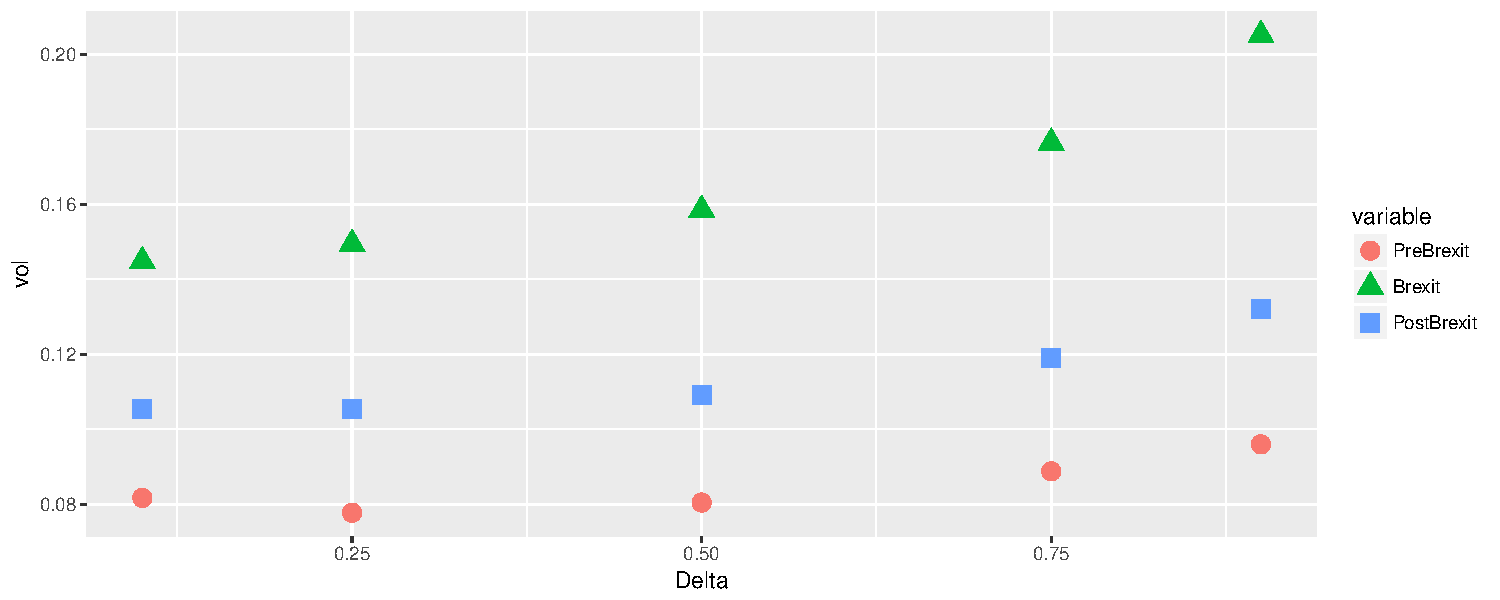
\includegraphics[width=1\linewidth]{2018_02_07_IMF_FXCourse_files/figure-beamer/unnamed-chunk-33-1}

\end{frame}

\begin{frame}[fragile]{A more refined volatility smile (1)}

\begin{Shaded}
\begin{Highlighting}[]
\CommentTok{# Fit second degree polynomial to smile}
\NormalTok{fit.Vol =}\StringTok{ }\ControlFlowTok{function}\NormalTok{(data.vol, data.delta,delta.range)}
\NormalTok{\{}
\NormalTok{  poly.fit =}\StringTok{ }\KeywordTok{lm}\NormalTok{(data.vol }\OperatorTok{~}\StringTok{ }\KeywordTok{poly}\NormalTok{(data.delta, }\DecValTok{2}\NormalTok{, }\DataTypeTok{raw=}\OtherTok{TRUE}\NormalTok{))  }

  \CommentTok{# Use fitted polynomial to interpolate Delta-Vol Curve}
\NormalTok{  delta.square =}\StringTok{ }\NormalTok{delta.range}\OperatorTok{*}\NormalTok{delta.range}
\NormalTok{  delta.interc =}\StringTok{ }\KeywordTok{rep}\NormalTok{(}\DecValTok{1}\NormalTok{,}\KeywordTok{length}\NormalTok{(delta.range))}
  
\NormalTok{  X =}\StringTok{ }\KeywordTok{cbind}\NormalTok{(delta.interc, delta.range, delta.square)}
\NormalTok{  iVolInterpol =}\StringTok{ }\KeywordTok{t}\NormalTok{(}\KeywordTok{t}\NormalTok{(X)}\OperatorTok{*}\NormalTok{poly.fit}\OperatorTok{$}\NormalTok{coefficients)}
\NormalTok{  iVolInterpol =}\StringTok{ }\KeywordTok{rowSums}\NormalTok{(iVolInterpol)}

  \KeywordTok{return}\NormalTok{(iVolInterpol)}
\NormalTok{\}}
\end{Highlighting}
\end{Shaded}

\end{frame}

\begin{frame}[fragile]{A more refined volatility smile (2)}

\begin{Shaded}
\begin{Highlighting}[]
\CommentTok{# Get the data points from the vol.smile data frame}
\NormalTok{data.delta =}\StringTok{ }\NormalTok{vol.smile}\OperatorTok{$}\NormalTok{Delta}
\NormalTok{data.vol  =}\StringTok{ }\NormalTok{vol.smile}\OperatorTok{$}\NormalTok{PreBrexit}

\CommentTok{# Interpolation and extrapolation range}
\NormalTok{delta.range =}\StringTok{ }\KeywordTok{seq}\NormalTok{(}\DataTypeTok{from=}\FloatTok{0.01}\NormalTok{, }\DataTypeTok{to =} \FloatTok{0.99}\NormalTok{, }\DataTypeTok{by=}\FloatTok{0.005}\NormalTok{)}

\CommentTok{# Obtain the volatility smiles}
\NormalTok{smile.preBrexit =}\KeywordTok{fit.Vol}\NormalTok{(vol.smile}\OperatorTok{$}\NormalTok{PreBrexit, data.delta, delta.range)}
\NormalTok{smile.Brexit    =}\KeywordTok{fit.Vol}\NormalTok{(vol.smile}\OperatorTok{$}\NormalTok{Brexit, data.delta, delta.range)}
\NormalTok{smile.postBrexit=}\KeywordTok{fit.Vol}\NormalTok{(vol.smile}\OperatorTok{$}\NormalTok{PostBrexit, data.delta, delta.range)}
\end{Highlighting}
\end{Shaded}

\end{frame}

\begin{frame}[fragile]{A more refined volatility smile (3)}

\begin{Shaded}
\begin{Highlighting}[]
\CommentTok{# Group the extended volatility smiles in a data frame}
\NormalTok{smile.df =}\StringTok{ }\KeywordTok{data.frame}\NormalTok{(delta.range, smile.preBrexit, }
\NormalTok{                      smile.Brexit, smile.postBrexit)}
\KeywordTok{rownames}\NormalTok{(smile.df) =}\StringTok{ }\OtherTok{NULL}
\KeywordTok{colnames}\NormalTok{(smile.df) =}\StringTok{ }\KeywordTok{c}\NormalTok{(}\StringTok{"Delta"}\NormalTok{,}\StringTok{"preBrexit"}\NormalTok{,}\StringTok{"Brexit"}\NormalTok{, }\StringTok{"postBrexit"}\NormalTok{)}

\CommentTok{# Create the chart}
\KeywordTok{library}\NormalTok{(reshape2)}
\NormalTok{smile.data =}\StringTok{ }\KeywordTok{melt}\NormalTok{(smile.df, }\DataTypeTok{id=}\StringTok{"Delta"}\NormalTok{)}
\KeywordTok{ggplot}\NormalTok{(}\DataTypeTok{data =}\NormalTok{ smile.data, }\KeywordTok{aes}\NormalTok{(}\DataTypeTok{x=}\NormalTok{Delta, }\DataTypeTok{y=}\NormalTok{value, }\DataTypeTok{colour=}\NormalTok{variable)) }\OperatorTok{+}
\StringTok{  }\KeywordTok{geom_line}\NormalTok{(}\DataTypeTok{size=}\DecValTok{1}\NormalTok{) }\OperatorTok{+}\StringTok{ }\KeywordTok{labs}\NormalTok{(}\DataTypeTok{y=}\StringTok{"vol"}\NormalTok{)}
\end{Highlighting}
\end{Shaded}

\end{frame}

\begin{frame}{A more refined volatility smile (4)}

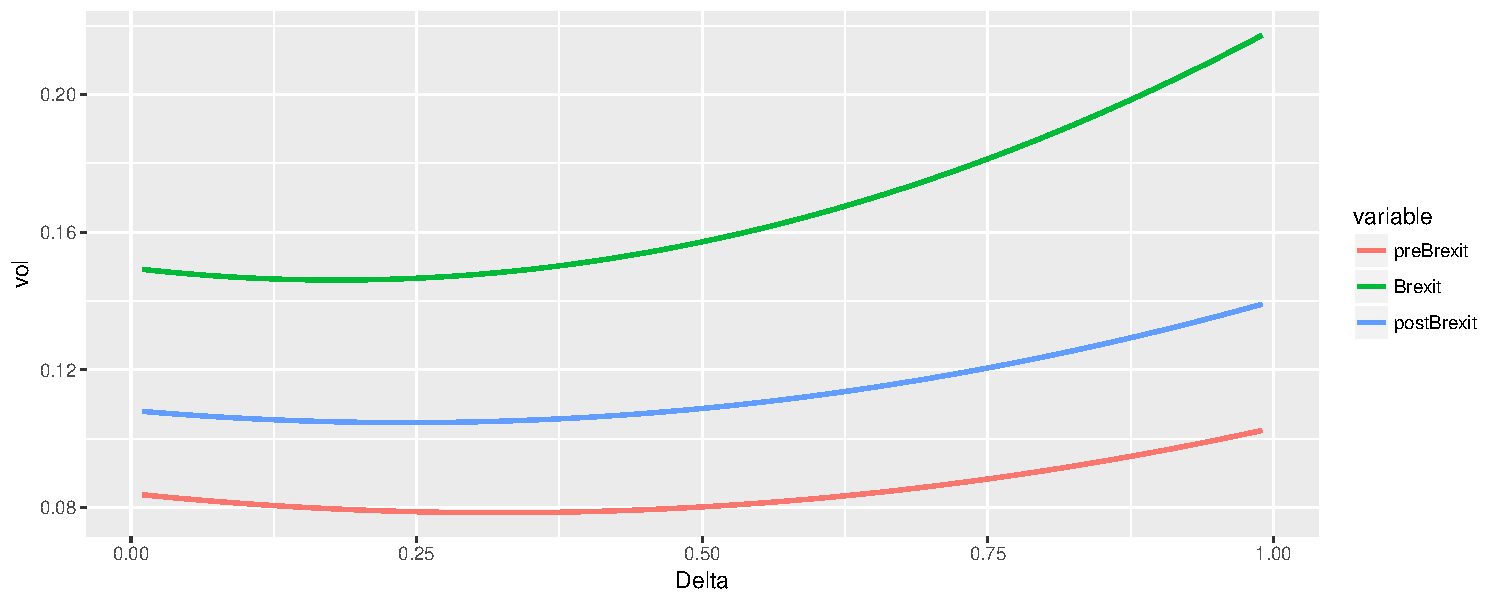
\includegraphics[width=1\linewidth]{2018_02_07_IMF_FXCourse_files/figure-beamer/unnamed-chunk-37-1}

\end{frame}

\begin{frame}{}

\color{blue} \LARGE{Part F:}\\
\LARGE{Extracting Risk-Neutral Densities}

\end{frame}

\begin{frame}{Market views are risk-neutral, not objective}

\end{frame}

\begin{frame}{Extraction methods}

Methods fall under one of three categories:

\begin{itemize}
\tightlist
\item
  Parametric methods
\item
  Semiparametric methods
\item
  Non-parametric methods
\end{itemize}

All methods require constructing call and/or put functions

\begin{itemize}
\tightlist
\item
  Option premia vs.~strike price
\end{itemize}

\end{frame}

\begin{frame}{Parametric methods}

\begin{itemize}
\tightlist
\item
  Specify a parametric distribution function \(F\) for the exchange rate
\item
  For the distribution parameters \(\Lambda\), the price of a call
  option is
\end{itemize}

\[
C^F(K) = \exp(-R_d\times T) \int_{K}^{\infty} \left( S_T - K\right) dF(S_T; \Lambda), 
\]

\begin{itemize}
\tightlist
\item
  The parameters that fit the market-implied distribution better solve
\end{itemize}

\[
\arg\min_{\Lambda} \sum_{j=1}^N |C^F(K_j) - C^{\text{Market}}(K_j)|^2
\]

\end{frame}

\begin{frame}{Semi-parametric methods}

\begin{itemize}
\tightlist
\item
  Start with a particular density
\item
  Add expansion terms to distribution
\item
  Each term helps to approximate market-implied distribution
\end{itemize}

\end{frame}

\begin{frame}{Non-parametric methods}

\begin{itemize}
\tightlist
\item
  Plot value of calls against different strike prices, i.e.
  \textbf{market call function}
\item
  Breeden and Litzenberger: risk-neutral distribution proportional to
  second derivative of the call function: \[
  \frac{\partial^2 C}{\partial K^2} \bigg\rvert_{K=S} = \exp(-R_d \times T)q(S).
  \]
\item
  Use numerical methods to calculate derivative and find risk neutral
  distribution
\end{itemize}

\end{frame}

\begin{frame}{}

\color{blue} \LARGE{Part F:}\\
\LARGE{Extracting Risk-Neutral Densities}\\
\Large{Constructing option premium functions}

\end{frame}

\begin{frame}[fragile]{Constructing the market call function (1)}

\begin{itemize}
\tightlist
\item
  We need to obtain the market call function
\item
  In other words, move from \(\Delta\) - \(\sigma\) space to
  \emph{Option premium} - \emph{Strike} space
\item
  Two useful functions in \texttt{auxFunctions.R}

  \begin{itemize}
  \tightlist
  \item
    \texttt{get.strike()}
  \item
    \texttt{GKoption.premium()}
  \end{itemize}
\end{itemize}

\end{frame}

\begin{frame}[fragile]{Constructing the market call function (2)}

\begin{Shaded}
\begin{Highlighting}[]
\NormalTok{get.strike =}\StringTok{ }\ControlFlowTok{function}\NormalTok{(vol,delta,S0,fwd,rf,Tenor)}
\NormalTok{\{}
\NormalTok{  aux =}\StringTok{ }\KeywordTok{qnorm}\NormalTok{(delta}\OperatorTok{*}\KeywordTok{exp}\NormalTok{(rf}\OperatorTok{*}\NormalTok{Tenor))}
\NormalTok{  aux =}\StringTok{ }\NormalTok{aux}\OperatorTok{*}\NormalTok{vol}\OperatorTok{*}\KeywordTok{sqrt}\NormalTok{(Tenor)}
\NormalTok{  aux =}\StringTok{ }\NormalTok{aux }\OperatorTok{-}\StringTok{ }\FloatTok{0.5}\OperatorTok{*}\NormalTok{vol}\OperatorTok{*}\NormalTok{vol}\OperatorTok{*}\NormalTok{Tenor}
\NormalTok{  K =}\StringTok{ }\KeywordTok{exp}\NormalTok{(}\OperatorTok{-}\NormalTok{aux)}\OperatorTok{*}\NormalTok{fwd}
  \KeywordTok{return}\NormalTok{(K)}
\NormalTok{\}}
\end{Highlighting}
\end{Shaded}

\end{frame}

\begin{frame}[fragile]{Constructing the market call function (3)}

\begin{Shaded}
\begin{Highlighting}[]
\NormalTok{GKoption.premium =}\StringTok{ }\ControlFlowTok{function}\NormalTok{(K,sigma,S,Tenor,fwd,rf,option_type)}
\NormalTok{\{}
  \ControlFlowTok{if}\NormalTok{ (option_type }\OperatorTok{==}\StringTok{"c"}\NormalTok{) \{w=}\DecValTok{1}\NormalTok{\}}
  \ControlFlowTok{if}\NormalTok{ (option_type }\OperatorTok{==}\StringTok{"p"}\NormalTok{) \{w=}\OperatorTok{-}\DecValTok{1}\NormalTok{\}}
\NormalTok{  d1 =}\StringTok{ }\KeywordTok{log}\NormalTok{(fwd}\OperatorTok{/}\NormalTok{K)}\OperatorTok{+}\FloatTok{0.5}\OperatorTok{*}\NormalTok{sigma}\OperatorTok{*}\NormalTok{sigma}\OperatorTok{*}\NormalTok{Tenor}
\NormalTok{  d1 =}\StringTok{ }\NormalTok{d1}\OperatorTok{/}\NormalTok{(sigma}\OperatorTok{*}\KeywordTok{sqrt}\NormalTok{(Tenor))}
\NormalTok{  d2 =}\StringTok{ }\NormalTok{d1 }\OperatorTok{-}\StringTok{ }\NormalTok{sigma}\OperatorTok{*}\KeywordTok{sqrt}\NormalTok{(Tenor)}
\NormalTok{  rd =}\StringTok{ }\KeywordTok{log}\NormalTok{(fwd}\OperatorTok{/}\NormalTok{S)}\OperatorTok{/}\NormalTok{Tenor }\OperatorTok{+}\StringTok{ }\NormalTok{rf}
\NormalTok{  premium =}\StringTok{ }\KeywordTok{exp}\NormalTok{(}\OperatorTok{-}\NormalTok{rd}\OperatorTok{*}\NormalTok{Tenor)}\OperatorTok{*}\NormalTok{(w}\OperatorTok{*}\NormalTok{fwd}\OperatorTok{*}\KeywordTok{pnorm}\NormalTok{(w}\OperatorTok{*}\NormalTok{d1) }\OperatorTok{-}\StringTok{ }\NormalTok{w}\OperatorTok{*}\NormalTok{K}\OperatorTok{*}\KeywordTok{pnorm}\NormalTok{(w}\OperatorTok{*}\NormalTok{d2))}
  \KeywordTok{return}\NormalTok{(premium)}
\NormalTok{\}}
\end{Highlighting}
\end{Shaded}

\end{frame}

\begin{frame}[fragile]{Constructing the market call function (3)}

Strike ranges for the selected dates:

\begin{Shaded}
\begin{Highlighting}[]
\NormalTok{K_preBrexit =}\StringTok{ }\KeywordTok{mapply}\NormalTok{(get.strike,smile.df}\OperatorTok{$}\NormalTok{preBrexit, smile.df}\OperatorTok{$}\NormalTok{Delta, }
                     \DataTypeTok{S0=}\NormalTok{spot[}\DecValTok{1}\NormalTok{], }\DataTypeTok{fwd=}\NormalTok{forward[}\DecValTok{1}\NormalTok{], }\DataTypeTok{rf=}\NormalTok{rf[}\DecValTok{1}\NormalTok{], }\DataTypeTok{Tenor=}\FloatTok{0.25}\NormalTok{)}
\NormalTok{K_Brexit    =}\StringTok{ }\KeywordTok{mapply}\NormalTok{(get.strike,smile.df}\OperatorTok{$}\NormalTok{Brexit, smile.df}\OperatorTok{$}\NormalTok{Delta, }
                     \DataTypeTok{S0=}\NormalTok{spot[}\DecValTok{2}\NormalTok{], }\DataTypeTok{fwd=}\NormalTok{forward[}\DecValTok{2}\NormalTok{], }\DataTypeTok{rf=}\NormalTok{rf[}\DecValTok{2}\NormalTok{], }\DataTypeTok{Tenor=}\FloatTok{0.25}\NormalTok{)}
\NormalTok{K_postBrexit=}\StringTok{ }\KeywordTok{mapply}\NormalTok{(get.strike,smile.df}\OperatorTok{$}\NormalTok{postBrexit, smile.df}\OperatorTok{$}\NormalTok{Delta, }
                     \DataTypeTok{S0=}\NormalTok{spot[}\DecValTok{3}\NormalTok{], }\DataTypeTok{fwd=}\NormalTok{forward[}\DecValTok{3}\NormalTok{], }\DataTypeTok{rf=}\NormalTok{rf[}\DecValTok{3}\NormalTok{], }\DataTypeTok{Tenor=}\FloatTok{0.25}\NormalTok{)}
\end{Highlighting}
\end{Shaded}

\end{frame}

\begin{frame}[fragile]{Constructing the market call function (4)}

Generate the call premia:

\begin{Shaded}
\begin{Highlighting}[]
\NormalTok{Call_preBrexit =}\StringTok{ }\KeywordTok{mapply}\NormalTok{(GKoption.premium, K_preBrexit, }
\NormalTok{                        smile.df}\OperatorTok{$}\NormalTok{preBrexit, }\DataTypeTok{S=}\NormalTok{spot[}\DecValTok{1}\NormalTok{],}\DataTypeTok{Tenor=}\NormalTok{Tenor,}
                        \DataTypeTok{fwd=}\NormalTok{forward[}\DecValTok{1}\NormalTok{],}\DataTypeTok{rf=}\NormalTok{rf[}\DecValTok{1}\NormalTok{], }\DataTypeTok{option_type=}\StringTok{"c"}\NormalTok{)}

\NormalTok{Call_Brexit =}\StringTok{ }\KeywordTok{mapply}\NormalTok{(GKoption.premium, K_Brexit, }
\NormalTok{                     smile.df}\OperatorTok{$}\NormalTok{Brexit, }\DataTypeTok{S=}\NormalTok{spot[}\DecValTok{2}\NormalTok{],}\DataTypeTok{Tenor=}\NormalTok{Tenor,}
                     \DataTypeTok{fwd=}\NormalTok{forward[}\DecValTok{2}\NormalTok{],}\DataTypeTok{rf=}\NormalTok{rf[}\DecValTok{2}\NormalTok{],}\DataTypeTok{option_type=}\StringTok{"c"}\NormalTok{)}

\NormalTok{Call_postBrexit =}\StringTok{ }\KeywordTok{mapply}\NormalTok{(GKoption.premium, K_postBrexit, }
\NormalTok{                         smile.df}\OperatorTok{$}\NormalTok{postBrexit,}\DataTypeTok{S=}\NormalTok{spot[}\DecValTok{3}\NormalTok{],}\DataTypeTok{Tenor=}\NormalTok{Tenor,}
                         \DataTypeTok{fwd=}\NormalTok{forward[}\DecValTok{3}\NormalTok{],}\DataTypeTok{rf=}\NormalTok{rf[}\DecValTok{3}\NormalTok{],}\DataTypeTok{option_type=}\StringTok{"c"}\NormalTok{)}
\end{Highlighting}
\end{Shaded}

\end{frame}

\begin{frame}[fragile]{Constructing the market call function (5)}

The data frame \texttt{callstrike.df} collects the call premium-strike
functions for the selected dates:

\begin{Shaded}
\begin{Highlighting}[]
\NormalTok{callstrike.df =}\StringTok{ }\KeywordTok{data.frame}\NormalTok{(K_preBrexit, Call_preBrexit, }
\NormalTok{                           K_Brexit, Call_Brexit, }
\NormalTok{                           K_postBrexit, Call_postBrexit)}
\end{Highlighting}
\end{Shaded}

\end{frame}

\begin{frame}[fragile]{Constructing the market call function (6)}

Plot the market call function

\begin{Shaded}
\begin{Highlighting}[]
\KeywordTok{ggplot}\NormalTok{(callstrike.df) }\OperatorTok{+}
\StringTok{  }\KeywordTok{geom_line}\NormalTok{(}\KeywordTok{aes}\NormalTok{(}\DataTypeTok{x=}\NormalTok{K_preBrexit,}\DataTypeTok{y=}\NormalTok{Call_preBrexit), }\DataTypeTok{col=}\StringTok{"red"}\NormalTok{, }\DataTypeTok{size=}\DecValTok{1}\NormalTok{) }\OperatorTok{+}\StringTok{ }
\StringTok{  }\KeywordTok{geom_line}\NormalTok{(}\KeywordTok{aes}\NormalTok{(}\DataTypeTok{x=}\NormalTok{K_Brexit, }\DataTypeTok{y=}\NormalTok{Call_Brexit), }\DataTypeTok{col=}\StringTok{"darkcyan"}\NormalTok{, }\DataTypeTok{size=}\DecValTok{1}\NormalTok{) }\OperatorTok{+}
\StringTok{  }\KeywordTok{geom_line}\NormalTok{(}\KeywordTok{aes}\NormalTok{(}\DataTypeTok{x=}\NormalTok{K_postBrexit, }\DataTypeTok{y=}\NormalTok{Call_postBrexit), }\DataTypeTok{col=}\StringTok{"blue"}\NormalTok{, }\DataTypeTok{size=}\DecValTok{1}\NormalTok{) }\OperatorTok{+}
\StringTok{  }\KeywordTok{labs}\NormalTok{(}\DataTypeTok{x=}\StringTok{"GBPUSD"}\NormalTok{, }\DataTypeTok{y=}\StringTok{"Strike price"}\NormalTok{) }\OperatorTok{+}\StringTok{ }
\StringTok{  }\KeywordTok{geom_vline}\NormalTok{(}\DataTypeTok{xintercept =}\NormalTok{ spot[}\DecValTok{1}\NormalTok{], }\DataTypeTok{col=}\StringTok{"red"}\NormalTok{, }\DataTypeTok{linetype=}\StringTok{"longdash"}\NormalTok{) }\OperatorTok{+}\StringTok{ }
\StringTok{  }\KeywordTok{geom_vline}\NormalTok{(}\DataTypeTok{xintercept =}\NormalTok{ spot[}\DecValTok{2}\NormalTok{], }\DataTypeTok{col=}\StringTok{"darkcyan"}\NormalTok{, }\DataTypeTok{linetype=}\StringTok{"longdash"}\NormalTok{) }\OperatorTok{+}
\StringTok{  }\KeywordTok{geom_vline}\NormalTok{(}\DataTypeTok{xintercept =}\NormalTok{ spot[}\DecValTok{3}\NormalTok{], }\DataTypeTok{col=}\StringTok{"blue"}\NormalTok{, }\DataTypeTok{linetype=}\StringTok{"longdash"}\NormalTok{) }\OperatorTok{+}
\StringTok{  }\KeywordTok{geom_hline}\NormalTok{(}\DataTypeTok{yintercept =} \DecValTok{0}\NormalTok{, }\DataTypeTok{col=}\StringTok{"black"}\NormalTok{)}
\end{Highlighting}
\end{Shaded}

\end{frame}

\begin{frame}{Constructing the market call function (7)}

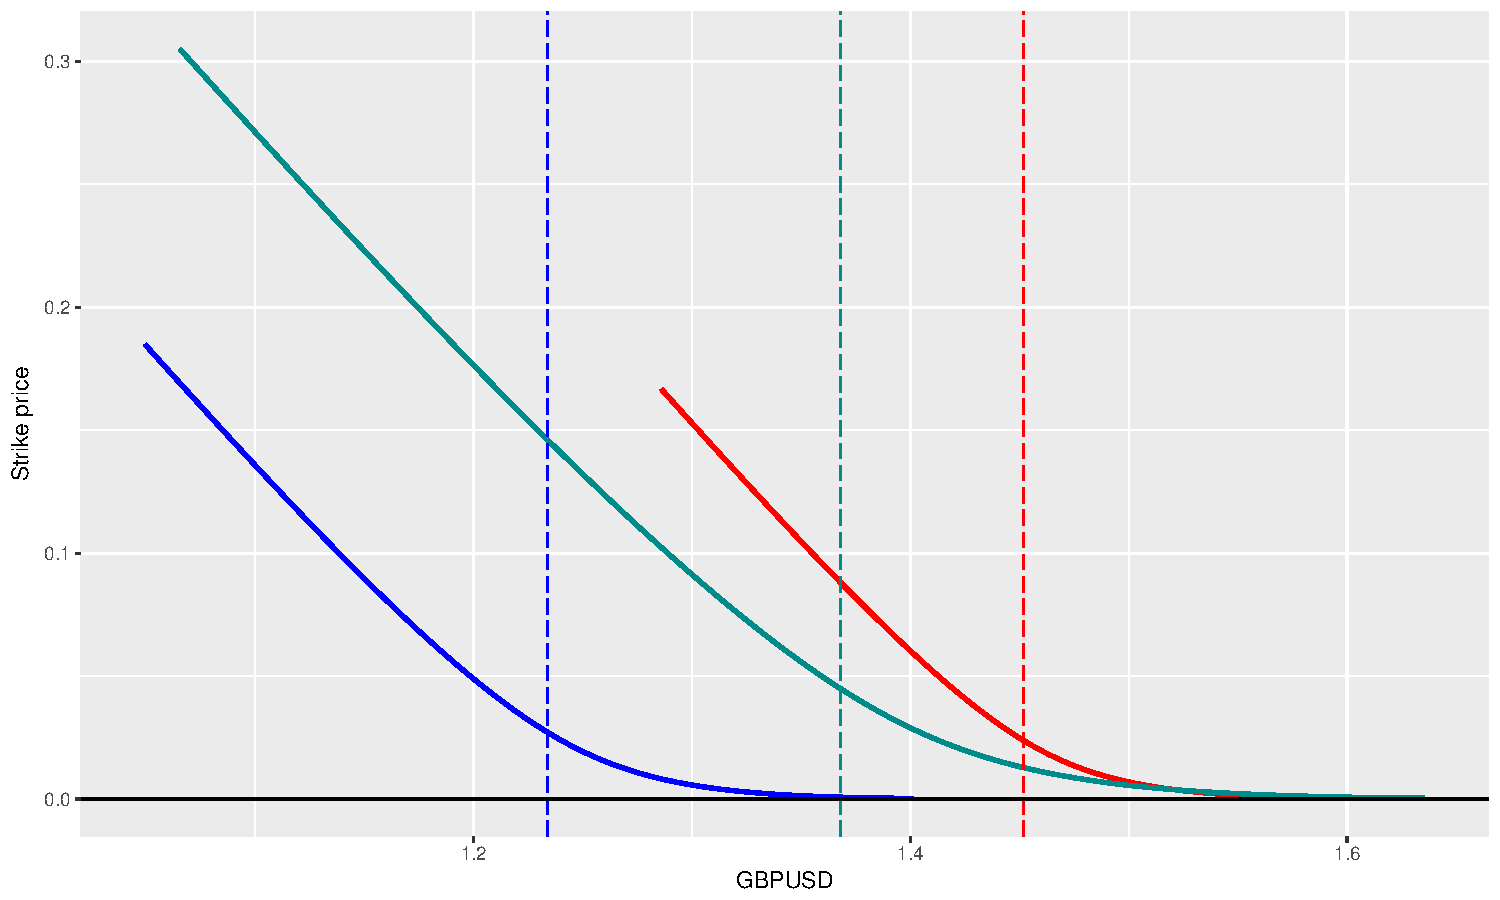
\includegraphics[width=0.9\linewidth]{2018_02_07_IMF_FXCourse_files/figure-beamer/unnamed-chunk-44-1}

\end{frame}

\begin{frame}{Constructing the market call function (8)}

Question: the call premium-strike functions are downward sloping,
i.e.~the call premium is higher for lower strike prices. Does this make
sense? Explain why.

\end{frame}

\begin{frame}[fragile]{Constructing the market put function (1)}

\begin{Shaded}
\begin{Highlighting}[]
\NormalTok{Put_preBrexit =}\StringTok{ }\KeywordTok{mapply}\NormalTok{(GKoption.premium, K_preBrexit, }
\NormalTok{                       smile.df}\OperatorTok{$}\NormalTok{preBrexit,}\DataTypeTok{S=}\NormalTok{spot[}\DecValTok{1}\NormalTok{],}\DataTypeTok{Tenor=}\NormalTok{Tenor,}
                       \DataTypeTok{fwd=}\NormalTok{forward[}\DecValTok{1}\NormalTok{],}\DataTypeTok{rf=}\NormalTok{rf[}\DecValTok{1}\NormalTok{],}\DataTypeTok{option_type=}\StringTok{"p"}\NormalTok{)}

\NormalTok{Put_Brexit =}\StringTok{ }\KeywordTok{mapply}\NormalTok{(GKoption.premium, K_Brexit, smile.df}\OperatorTok{$}\NormalTok{Brexit,}
                        \DataTypeTok{S=}\NormalTok{spot[}\DecValTok{2}\NormalTok{],}\DataTypeTok{Tenor=}\NormalTok{Tenor,}\DataTypeTok{fwd=}\NormalTok{forward[}\DecValTok{2}\NormalTok{],}
                        \DataTypeTok{rf=}\NormalTok{rf[}\DecValTok{2}\NormalTok{],}\DataTypeTok{option_type=}\StringTok{"p"}\NormalTok{)}

\NormalTok{Put_postBrexit =}\StringTok{ }\KeywordTok{mapply}\NormalTok{(GKoption.premium, K_postBrexit, }
\NormalTok{                        smile.df}\OperatorTok{$}\NormalTok{postBrexit,}\DataTypeTok{S=}\NormalTok{spot[}\DecValTok{3}\NormalTok{],}\DataTypeTok{Tenor=}\NormalTok{Tenor,}
                        \DataTypeTok{fwd=}\NormalTok{forward[}\DecValTok{3}\NormalTok{],}\DataTypeTok{rf=}\NormalTok{rf[}\DecValTok{3}\NormalTok{],}\DataTypeTok{option_type=}\StringTok{"p"}\NormalTok{)}
\end{Highlighting}
\end{Shaded}

\end{frame}

\begin{frame}[fragile]{Constructing the market put function (2)}

\begin{Shaded}
\begin{Highlighting}[]
\NormalTok{putstrike.df =}\StringTok{ }\KeywordTok{data.frame}\NormalTok{(K_preBrexit, Put_preBrexit, }
\NormalTok{                          K_Brexit, Put_Brexit, }
\NormalTok{                          K_postBrexit, Put_postBrexit)}
\end{Highlighting}
\end{Shaded}

\end{frame}

\begin{frame}[fragile]{Constructing the market put function (3)}

\begin{Shaded}
\begin{Highlighting}[]
\KeywordTok{ggplot}\NormalTok{(putstrike.df) }\OperatorTok{+}\StringTok{ }
\StringTok{  }\KeywordTok{geom_line}\NormalTok{(}\KeywordTok{aes}\NormalTok{(}\DataTypeTok{x=}\NormalTok{K_preBrexit,}\DataTypeTok{y=}\NormalTok{Put_preBrexit), }\DataTypeTok{col=}\StringTok{"red"}\NormalTok{, }\DataTypeTok{size=}\DecValTok{1}\NormalTok{) }\OperatorTok{+}\StringTok{ }
\StringTok{  }\KeywordTok{geom_line}\NormalTok{(}\KeywordTok{aes}\NormalTok{(}\DataTypeTok{x=}\NormalTok{K_Brexit, }\DataTypeTok{y=}\NormalTok{Put_Brexit), }\DataTypeTok{col=}\StringTok{"darkcyan"}\NormalTok{, }\DataTypeTok{size=}\DecValTok{1}\NormalTok{) }\OperatorTok{+}
\StringTok{  }\KeywordTok{geom_line}\NormalTok{(}\KeywordTok{aes}\NormalTok{(}\DataTypeTok{x=}\NormalTok{K_postBrexit, }\DataTypeTok{y=}\NormalTok{Put_postBrexit), }\DataTypeTok{col=}\StringTok{"blue"}\NormalTok{, }\DataTypeTok{size=}\DecValTok{1}\NormalTok{) }\OperatorTok{+}
\StringTok{  }\KeywordTok{labs}\NormalTok{(}\DataTypeTok{x=}\StringTok{"Strike price"}\NormalTok{, }\DataTypeTok{y=}\StringTok{"Put premium"}\NormalTok{) }\OperatorTok{+}\StringTok{ }
\StringTok{  }\KeywordTok{geom_vline}\NormalTok{(}\DataTypeTok{xintercept =}\NormalTok{ spot[}\DecValTok{1}\NormalTok{], }\DataTypeTok{col=}\StringTok{"red"}\NormalTok{, }\DataTypeTok{linetype=}\StringTok{"longdash"}\NormalTok{) }\OperatorTok{+}\StringTok{ }
\StringTok{  }\KeywordTok{geom_vline}\NormalTok{(}\DataTypeTok{xintercept =}\NormalTok{ spot[}\DecValTok{2}\NormalTok{], }\DataTypeTok{col=}\StringTok{"darkcyan"}\NormalTok{, }\DataTypeTok{linetype=}\StringTok{"longdash"}\NormalTok{) }\OperatorTok{+}
\StringTok{  }\KeywordTok{geom_vline}\NormalTok{(}\DataTypeTok{xintercept =}\NormalTok{ spot[}\DecValTok{3}\NormalTok{], }\DataTypeTok{col=}\StringTok{"blue"}\NormalTok{, }\DataTypeTok{linetype=}\StringTok{"longdash"}\NormalTok{) }\OperatorTok{+}
\StringTok{  }\KeywordTok{geom_hline}\NormalTok{(}\DataTypeTok{yintercept =} \DecValTok{0}\NormalTok{, }\DataTypeTok{col=}\StringTok{"black"}\NormalTok{)}
\end{Highlighting}
\end{Shaded}

\end{frame}

\begin{frame}{Constructing the market put function (4)}

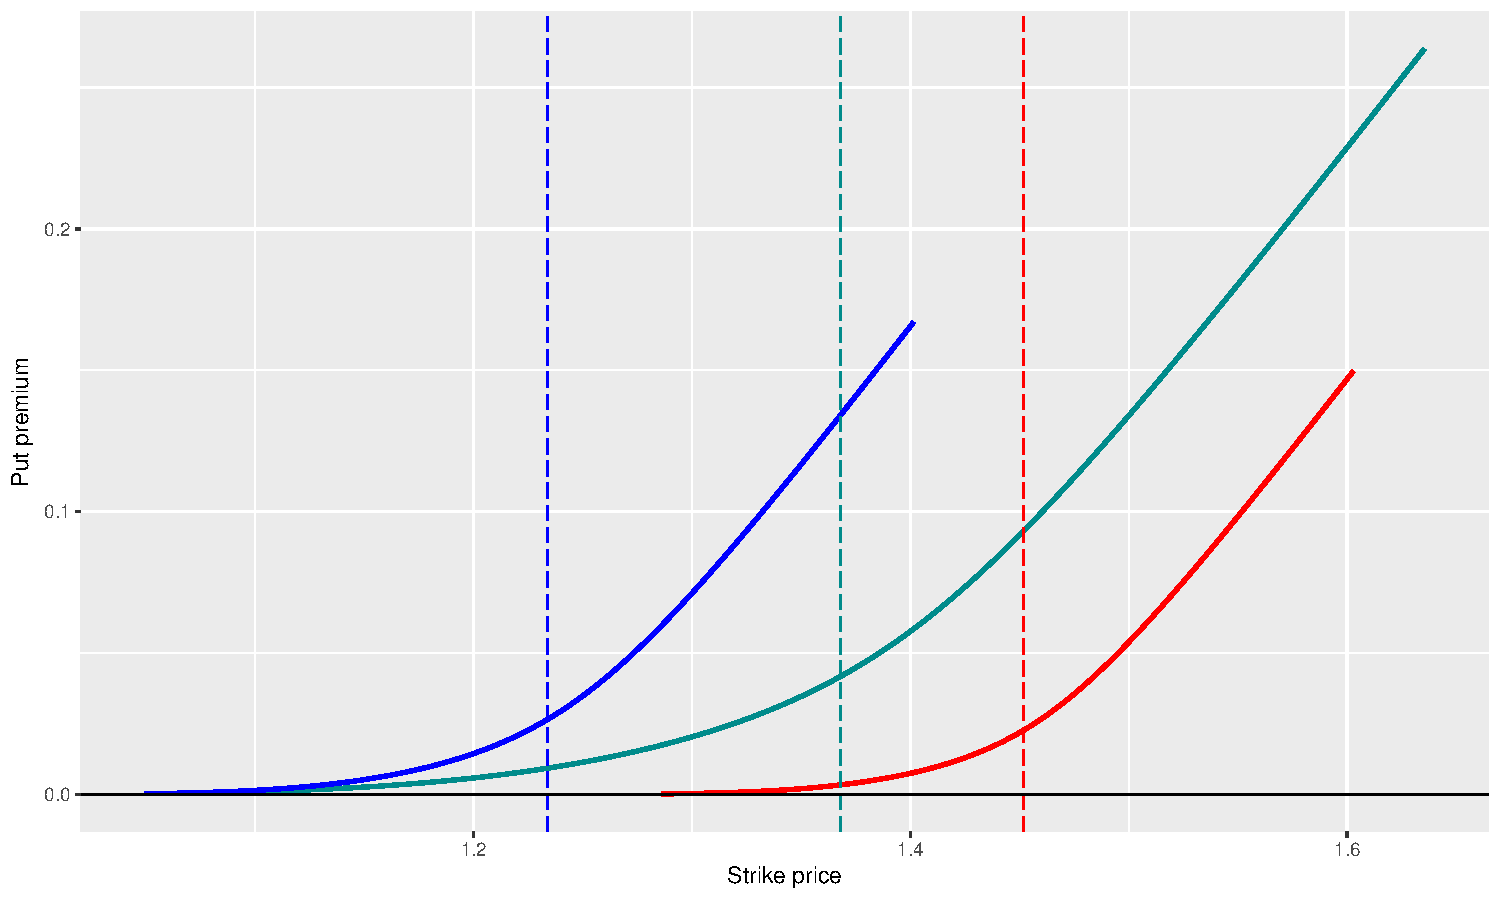
\includegraphics[width=0.9\linewidth]{2018_02_07_IMF_FXCourse_files/figure-beamer/unnamed-chunk-48-1}

\end{frame}

\begin{frame}{}

\color{blue} \LARGE{Part F:}\\
\LARGE{Extracting Risk-Neutral Densities}\\
\Large{Using the RND package to generate densities}

\end{frame}
